%!TEX root = widefieldscan.tex
\svnidlong
{$HeadURL$}
{$LastChangedDate$}
{$LastChangedRevision$}
{$LastChangedBy$}

\begin{center}
	\fbox{
		\begin{minipage}{.618\columnwidth}
		The section below is versioned at \url{\svnkw{HeadURL}} (last commit @ \svnfileday.\svnfilemonth.\svnfileyear \space \svnfilehour:\svnfileminute, Revision: \svnkw{LastChangedRevision}).
		\end{minipage}
	} 
\end{center}

\section{Results}
\label{sec:Results}
\subsection{Image Merging and Reconstruction}
\label{sec:Image Merging and Reconstruction}
Results of the steps mentioned in section~\ref{sec:materials and methods} are shown in figure~\ref{fig:wide field scan results}. Figure~\ref{fig:subscans} shows exemplary projection images from overlapping subscans prior to correction and normalization. Figure~\ref{fig:merge-proj} shows a merged projection image prior to reconstruction and figure~\ref{fig:merge-rec} shows the end-result of such a wide field scan, a reconstructed slice of the whole sample with a FOV of \SI{2994}{pixels} (\SI{4.19}{\milli\meter}) which is approximately three times the size of what can be achieved with one single binned scan (\SI{1024}{pixels} or \SI{1.43}{\milli\meter}).

\begin{figure*}
	\renewcommand{\imsize}{.16\linewidth}
	\pgfmathsetlength{\imagewidth}{\imsize} % desired display width of image
	\pgfmathsetlength{\imagescale}{\imagewidth/512} % pixel width of image
	\centering
		\subfloat[Uncorrected projection images from subscans s$_1$--s$_3$, each with a size of 1024$\times$1024 pixels at a resolution of \SI{1.4}{\micro\meter\per pixel}, covering a FOV of approximately \SI{0.7}{\milli\meter}. The scans overlap each other by approximately 100 pixels. 4676 projections have been acquired for the subscans s$_1$ and s$_3$, 1169 projections have been acquired for subscan s$_2$, all over a rotation of \SI{180}{\degree}.]{%
			\label{fig:s1}%
			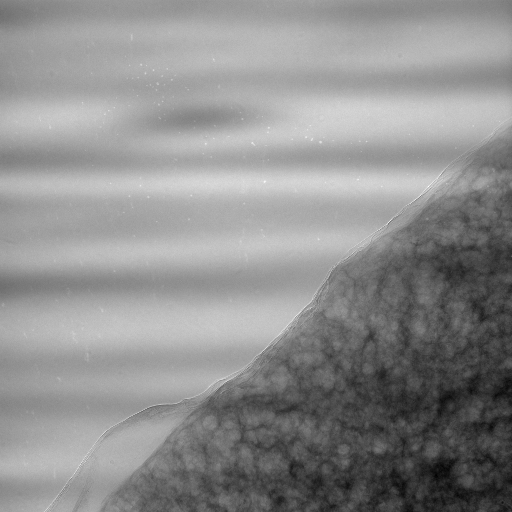
\includegraphics[width=\imsize]{img/merge/R108C10B-s1}%
			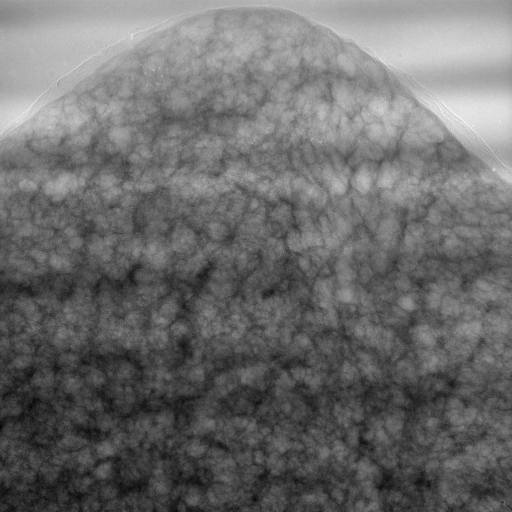
\includegraphics[width=\imsize]{img/merge/R108C10B-s2}%
			\begin{tikzpicture}[x=\imagescale,y=-\imagescale]
				% place image (integer coordinates refer to pixel centers):
				\node[anchor=north west,inner sep=0pt,outer sep=0pt] at (0,0)
					{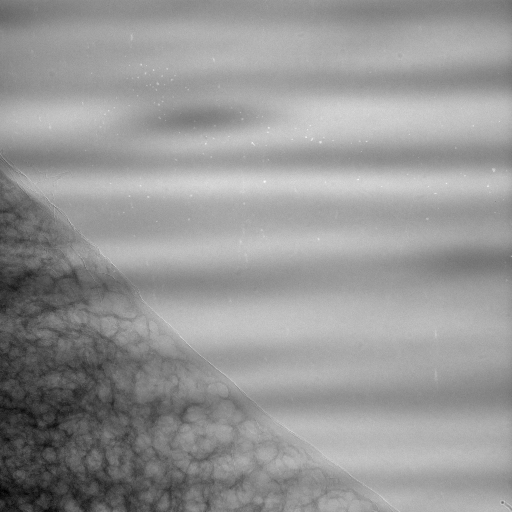
\includegraphics[width=\imagewidth]{img/merge/R108C10B-s3}};
				\draw[|-|,color=white] (256-64,450) -- (512-64,450) node[midway,above] {\SI{700}{\micro\meter}};
			\end{tikzpicture}
			\label{fig:subscans}
			}
		\renewcommand{\imsize}{.48\linewidth}
		\pgfmathsetlength{\imagewidth}{\imsize} % desired displayed width of image
		\pgfmathsetlength{\imagescale}{\imagewidth/1498} % pixel width of image
		\subfloat[Merged and corrected image from the three subscans shown in subfigure~\subref{fig:subscans}. The merged projections have a size of 2994$\times$1024 pixels at a resolution of \SI{1.4}{\micro\meter\per pixel}. The Subscans s$_1$--s$_3$ overlap each other by approximately 150 pixels. The width of the merged projections is thus smaller than three times the width of the subscans.]{%
			\begin{tikzpicture}[x=\imagescale,y=-\imagescale]
				\node[anchor=north west,inner sep=0pt,outer sep=0pt] at (0,0)
					{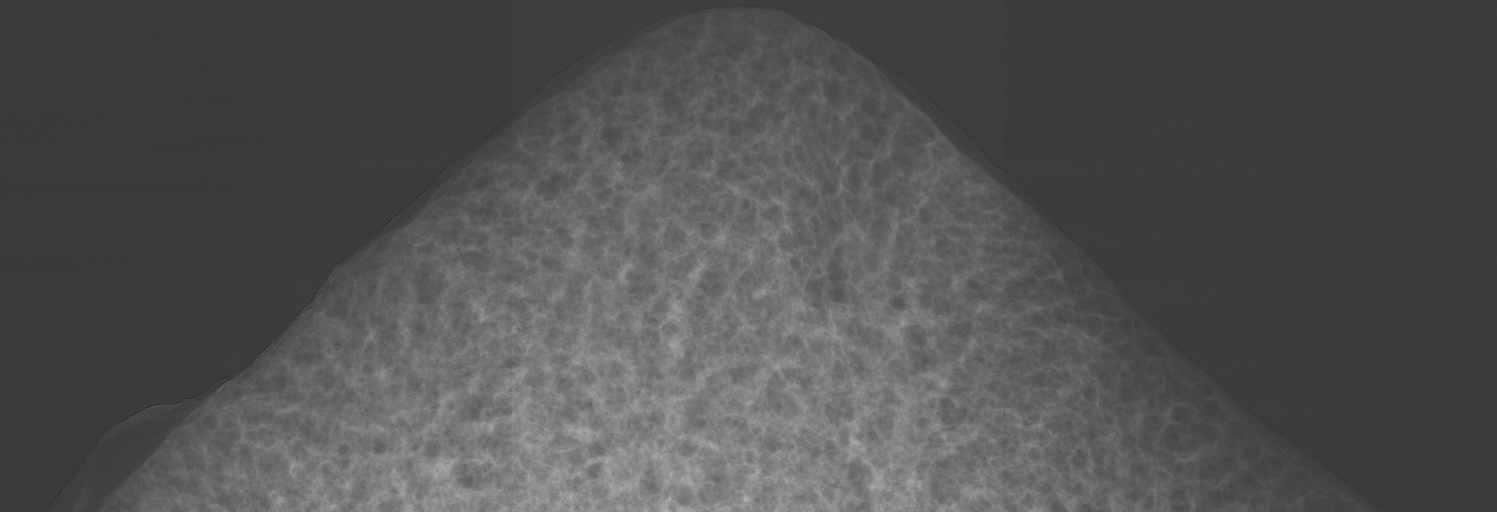
\includegraphics[width=\imagewidth]{img/merge/R108C10B-merge}};
				\draw[|-|,color=white] (1242-64,450) -- (1498-64,450) node[midway,above] {\SI{700}{\micro\meter}};
			\end{tikzpicture}
			\label{fig:merge-proj}
			}
		\renewcommand{\imsize}{\linewidth}
		\pgfmathsetlength{\imagewidth}{\imsize} % desired displayed width of image
		\pgfmathsetlength{\imagescale}{\imagewidth/1365} % pixel width of image (image has been resized from 2994*1123, so that scalebar is at the same height without calculating too much...)
		\subfloat[Cropped part of one slice of the tomographic dataset reconstructed from the merged projections, where one is shown in subfigure~\subref{fig:merge-proj}. The halo directly around the lung tissue arises from the paraffin where the sample is embedded in. The bright circular shape inscribed in the square arises from the filtered back-projection, the chosen reconstruction method. The size of the cropped image is 2994$\times$1123 pixels. The inset shows an overview over the full slice with a size of 2994$\times$2994 pixels.]{%
			\begin{tikzpicture}[x=\imagescale,y=-\imagescale]
				% place image (integer coordinates refer to pixel centers):
				\node[anchor=north west,inner sep=0pt,outer sep=0pt] at (0,0)
					{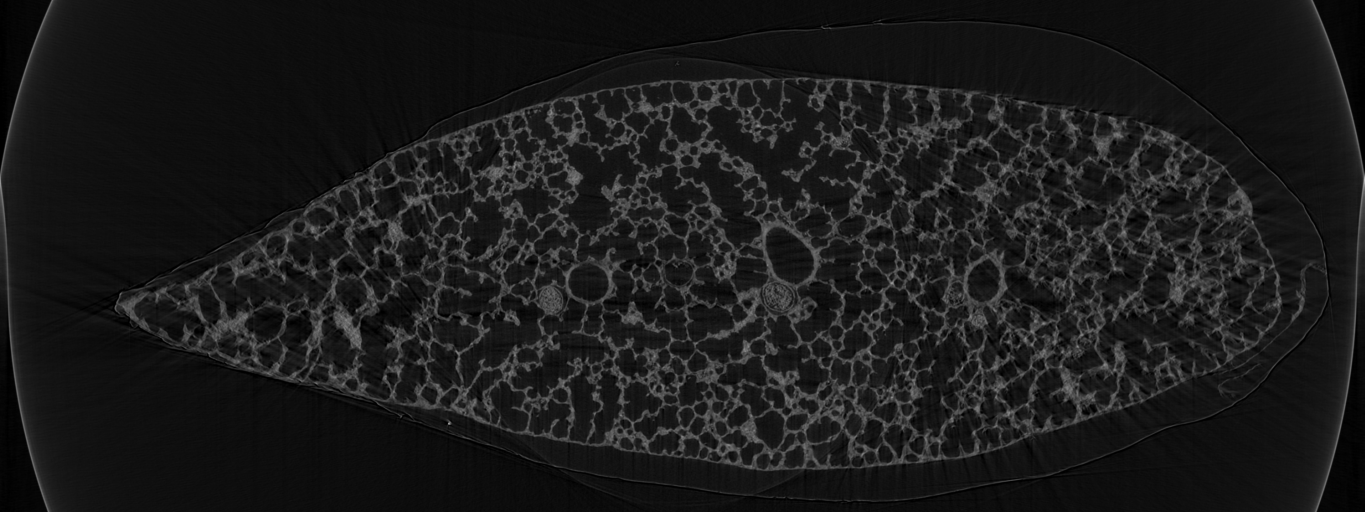
\includegraphics[width=\imagewidth]{img/merge/R108C10B-merge1016-crop}};
				\newcommand{\size}{.2\imagewidth}
				\node[anchor=north west,inner sep=0pt,outer sep=0pt] at (0,0)
					{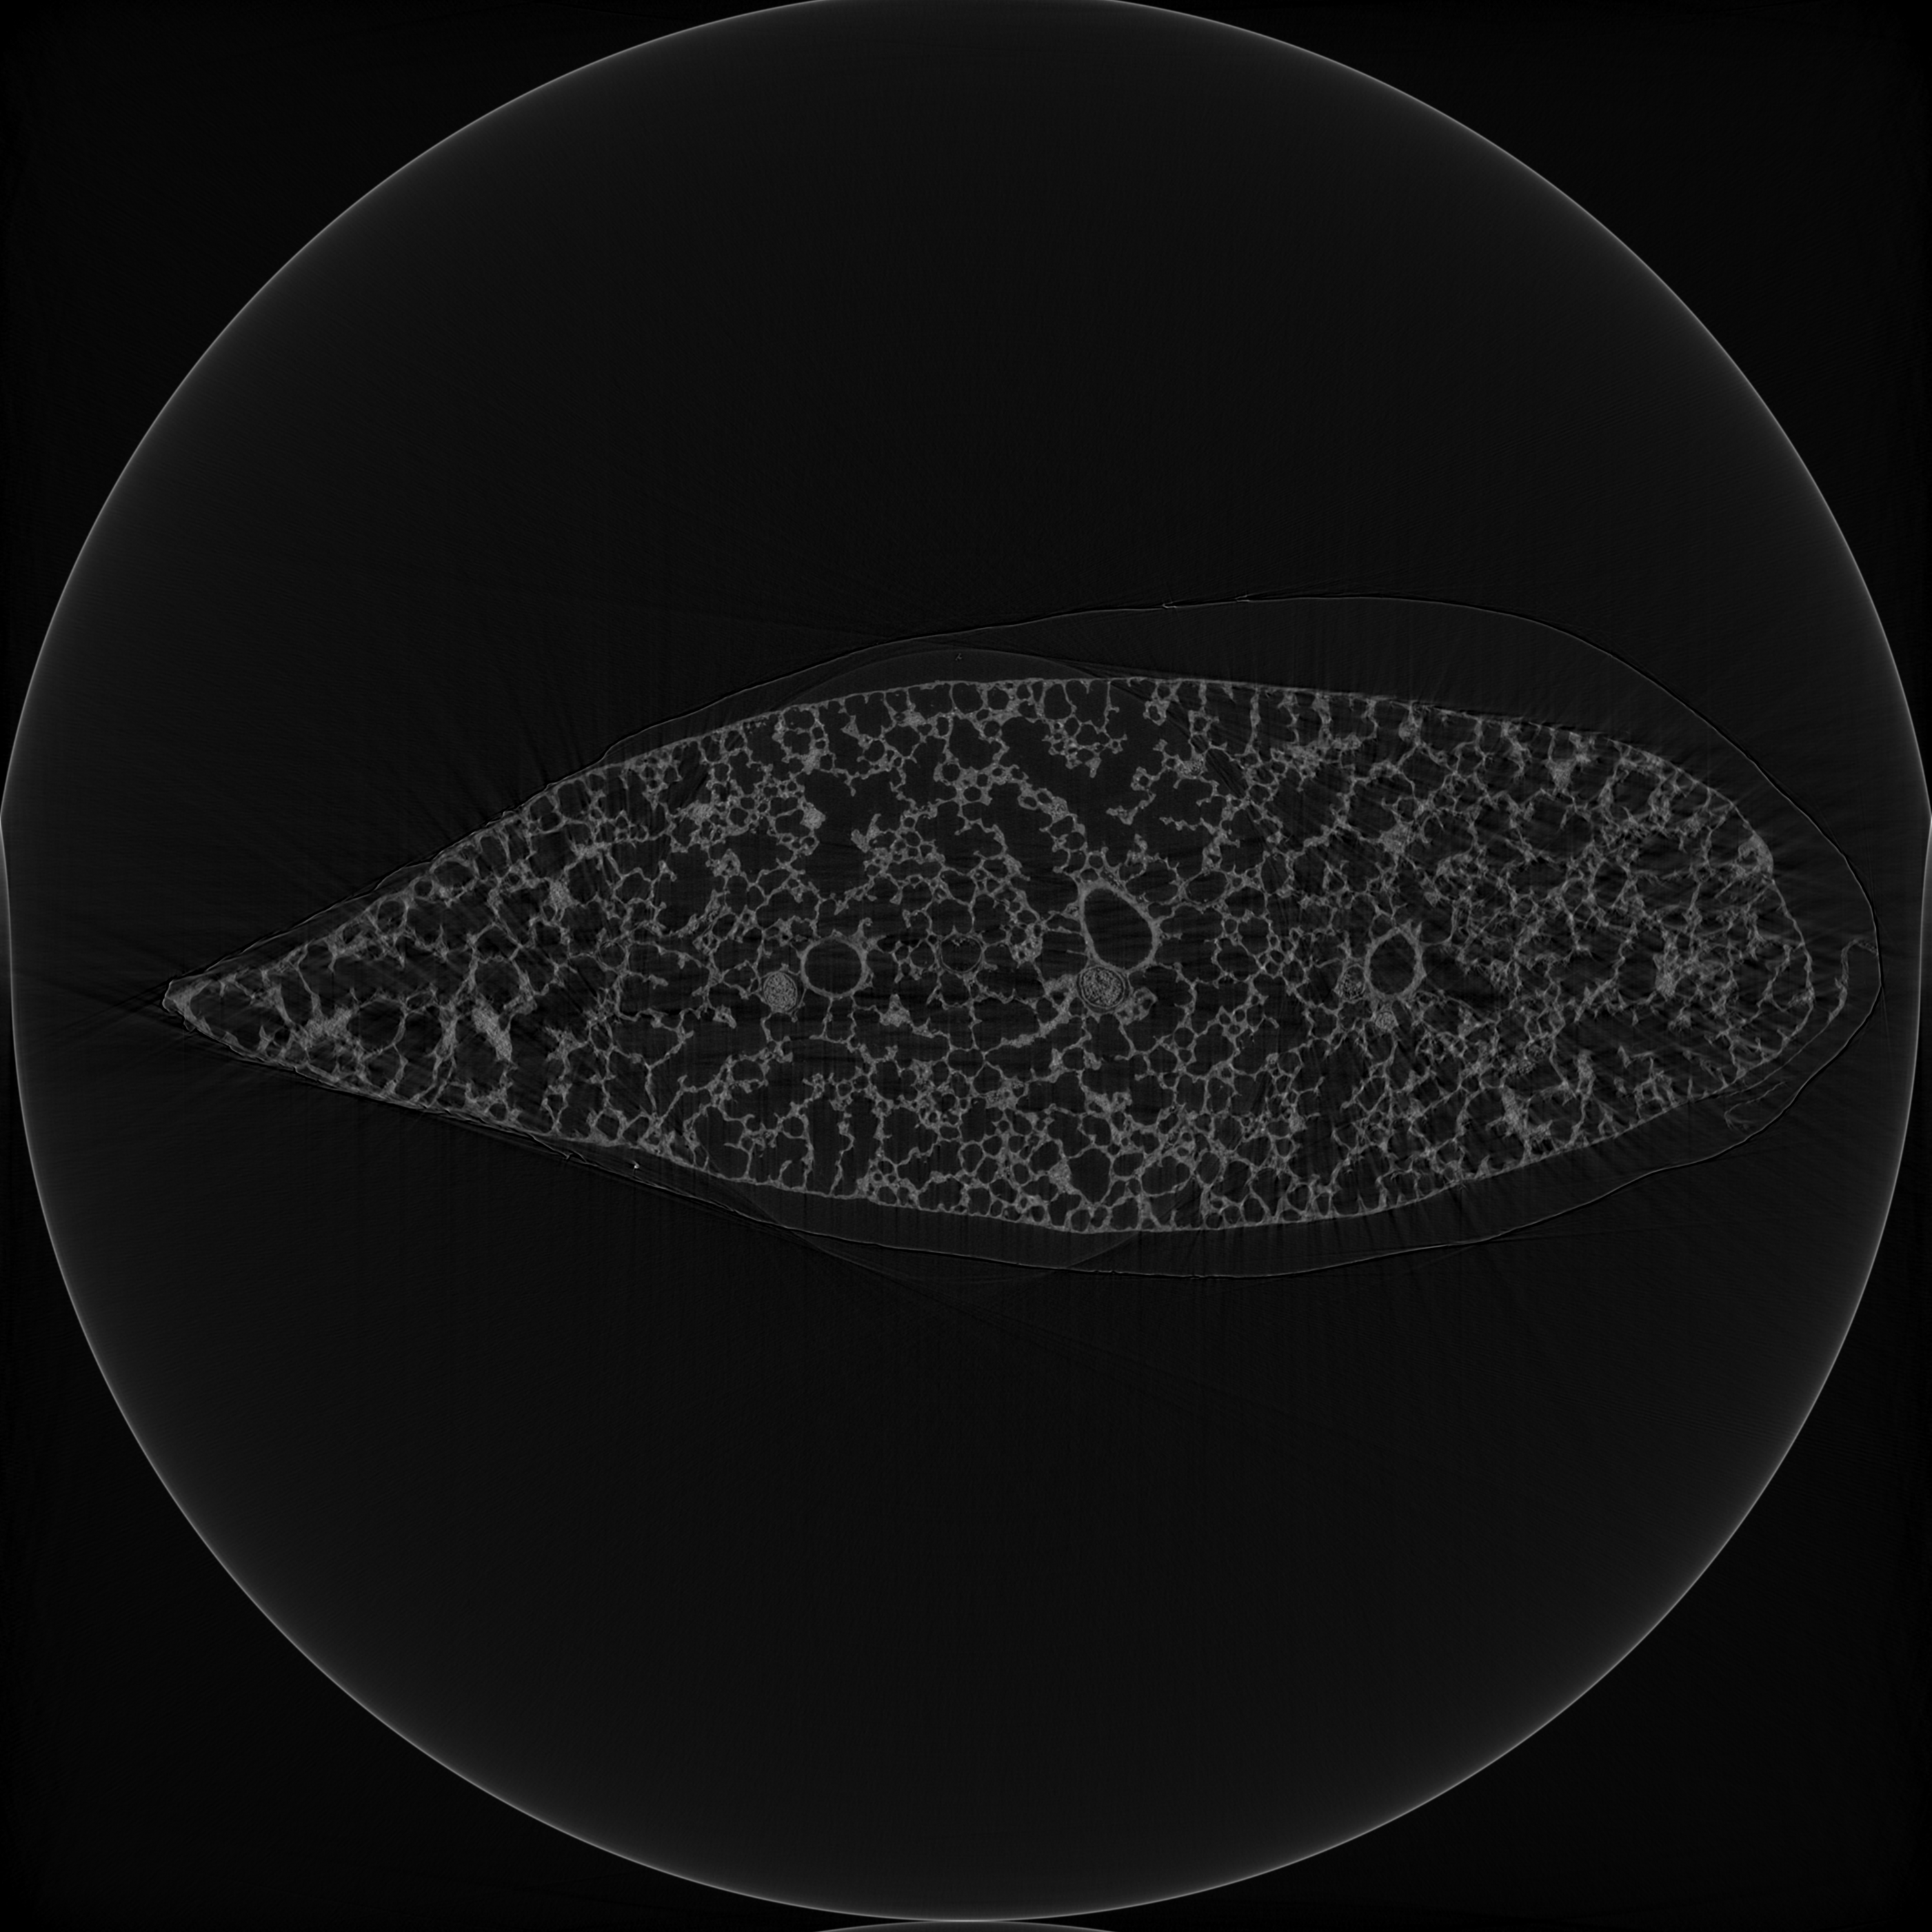
\includegraphics[width=\size]{img/merge/R108C10B-merge1016}};
					\draw[white] (\size,0) -- (\size,-\size) -- (0,-\size);
				\draw[|-|,color=white] (1109-64,450) -- (1365-64,450) node[midway,above] {\SI{700}{\micro\meter}};
			\end{tikzpicture}
			\label{fig:merge-rec}
			}
	\caption{Different stages of a wide field scan of a rat lung sample obtained from a Sprague-Dawley rat 10 days after birth, showing the distal-medial edge of the right lower lung lobe. The sample has been scanned at a beam energy of \SI{12.6}{\kilo\electronvolt}.}
	\label{fig:wide field scan results}	
\end{figure*}

\subsection{Increasing the FOV}
The desire to increase the FOV of tomographic datasets at TOMCAT has arisen with the need to obtain high resolution three dimensional data of the terminal airways in the lung. As stated in section~\ref{subsec:motivation} we are interested in detecting and visualizing entire acini over the course of the postnatal lung development in mammals. To be able to study these functional lung units we need the high resolution that TOMCAT is able to provide\todo{explain why we actually need it $\rightarrow$ border where change from ``luftleitend'' to ``gasaustausch'' happens, septal thickness, etc.}. With the FOV available up to now at TOMCAT we have only been able to fit partial acini inside our datasets. Increasing the available FOV approximately three times permits us to obtain three dimensional reconstructions of entire acini which are only restricted by sample size, but not by the FOV of the imaging method. When comparing the green and red airway segments in figures~\ref{fig:FOV increase overview} and \ref{fig:FOV increase segments} with each other, we can see that with the conventional tomographic imaging, both segments are only partially in the FOV. We need to increase the FOV to be able to see the full central acinus inside the lung tissue. With the increased FOV we additionally see a third acinus (yellow segment) inside the lung segment. Both the red and yellow segment are only partial acini, but their size is limited by the dimensions of the lung sample, not by the FOV. The cutting lines are visible in the underside view of the wide field scanning visualization (Figure~\ref{subfig:down-merge}).

Both aforementioned figures show, that we have been able to increase the FOV of TOMCAT in such a way that we are now able to obtain tomographic datasets of entire acini of rat lungs. We plan to use this now available data to gain a deep insight into the postnatal structural lung development, see section~\ref{sec:outlook} for details.

\renewcommand{\imsize}{.5\linewidth}
\pgfmathsetlength{\imagewidth}{\imsize} % desired displayed width of image
\pgfmathsetlength{\imagescale}{\imagewidth/1202} % pixel width of imagefile used below
\begin{figure*}
	\centering
		\subfloat[conventional scan]{%
			\label{subfig:overview-s2}%
				\begin{tikzpicture}[x=\imagescale,y=-\imagescale]%
				\def\x{225}%
				\def\y{625}%
    				\node[anchor=north west,inner sep=0pt,outer sep=0pt] at (0,0)%
	    			{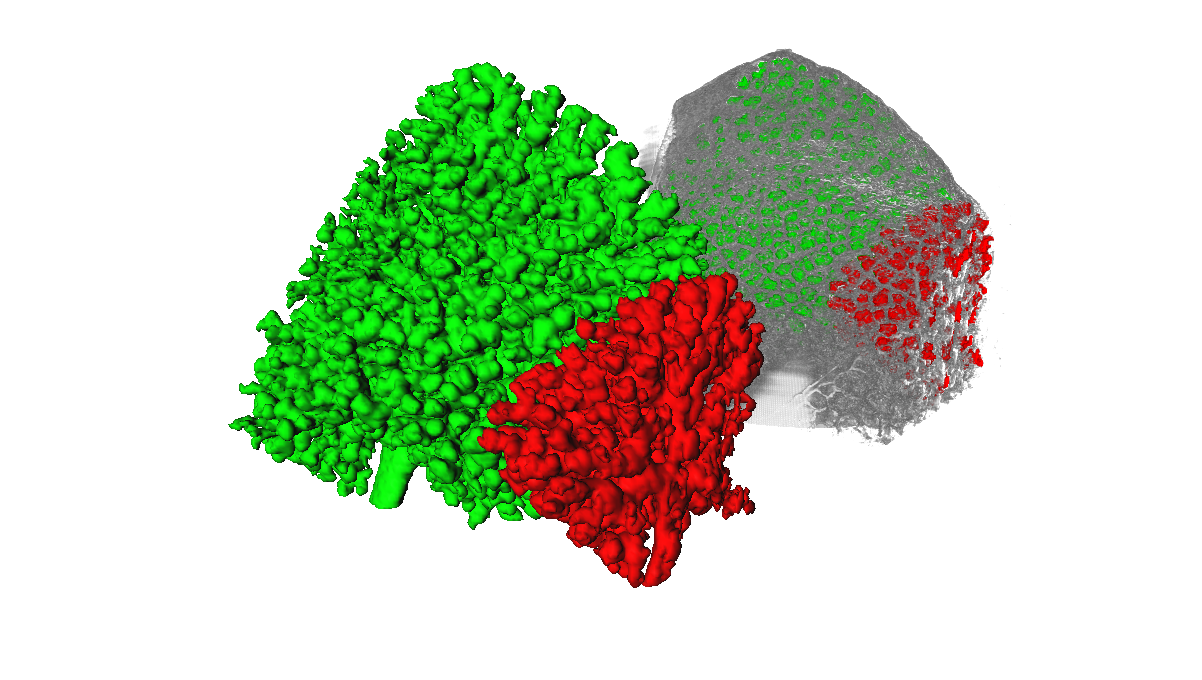
\includegraphics[width=\imagewidth]{img/widefieldscanning/R108C04C-overview-s2}};%
					\draw[|-|,thick] (229,428) -- (659,586) node [right] {\SI{1.4336}{\milli\meter}};%
%				    % 458 px = 1.4336 mm > 100 px = 313 um > 160 px = 500 um
				    \draw[|-|,thick] (\x,\y) -- (160+\x,\y) node [midway,above] {\SI{500}{\micro\meter}};%
				\end{tikzpicture}%
		}%
		\subfloat[wide field scan]{%
			\label{subfig:overview-merge}%
				\begin{tikzpicture}[x=\imagescale,y=-\imagescale]%
				\def\x{200}%
				\def\y{625}%
    				\node[anchor=north west,inner sep=0pt,outer sep=0pt] at (0,0)%
	    			{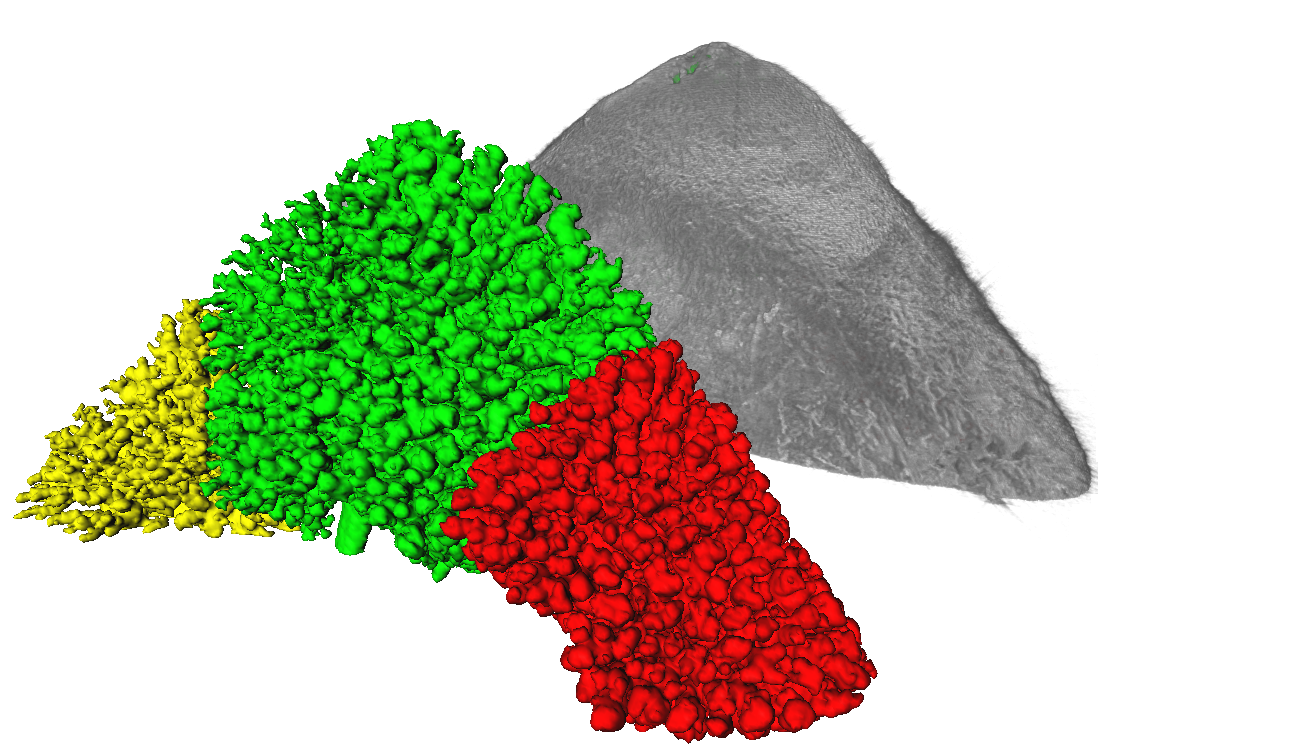
\includegraphics[width=\imagewidth]{img/widefieldscanning/R108C04C-overview-merge}};%
					\draw[|-|,thick] (40,456) -- (890,610) node [right] {\SI{3.8444}{\milli\meter}};%
				    % 864 px = 3.8444 mm > 100 px = 445 um > 112 px = 500 um
					\draw[|-|,thick] (\x,\y) -- (224+\x,\y) node [midway,above] {\SI{1}{\milli\meter}};%
				\end{tikzpicture}%
		}%
		\caption{Three dimensional visualization of the distal-medial edge of the right lower lung lobe of a Sprague Dawley rat. The grey structure in the background shows a semitransparent view of the sample with segmented airways. The foreground shows isosurfaces of terminal airways that have been extracted using a region growing algorithm (green and red for \subref{subfig:overview-s2}, green and red yellow for \subref{subfig:overview-merge}.}%
	\label{fig:FOV increase overview}%
	\todo[inline]{Do we need to add original slices to clearly show the increase in the FOV, or is this clear enough? Scale bars for this and ALL subsequent images are not finalized, need to be adjusted to sensible lengths.}
\end{figure*}

\renewcommand{\imsize}{.5\linewidth}
\pgfmathsetlength{\imagewidth}{\imsize} % desired displayed width of image
\pgfmathsetlength{\imagescale}{\imagewidth/1299} % pixel width of imagefile used below
\begin{figure*}
	\centering
		\subfloat[conventional scan]{%
			\label{subfig:down-s2}%
				\begin{tikzpicture}[x=\imagescale,y=-\imagescale]%
				\def\x{750}%
				\def\y{725}%
    				\node[anchor=north west,inner sep=0pt,outer sep=0pt] at (0,0)%
    				{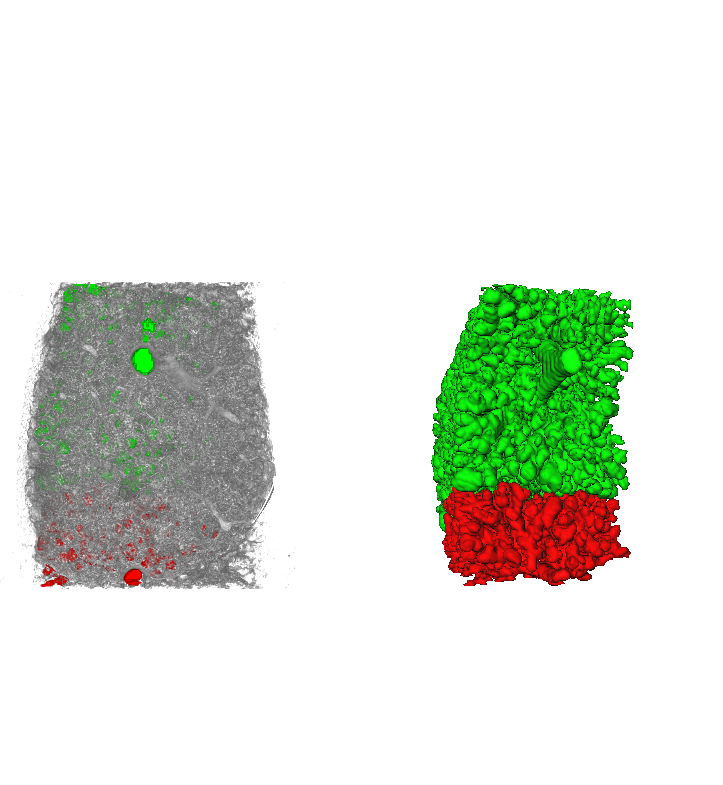
\includegraphics[width=\imagewidth]{img/widefieldscanning/R108C04C-down-s2}};%
				\draw[|-|,thick] (350,290) -- (350,595) node [left] {\SI{1.4336}{\milli\meter}};%
			   	 % 305 px = 1.4336 mm > 100 px = 470 um > 106 px = 500um
					\draw[|-|,thick] (\x,\y) -- (106+\x,+\y) node [midway,above] {\SI{500}{\micro\meter}};%
				\end{tikzpicture}%
		}%\\%
		\subfloat[wide field scan]{%
			\label{subfig:down-merge}%%
				\begin{tikzpicture}[x=\imagescale,y=-\imagescale]%
				\def\x{775}%
				\def\y{825}%
    				\node[anchor=north west,inner sep=0pt,outer sep=0pt] at (0,0)%
    				{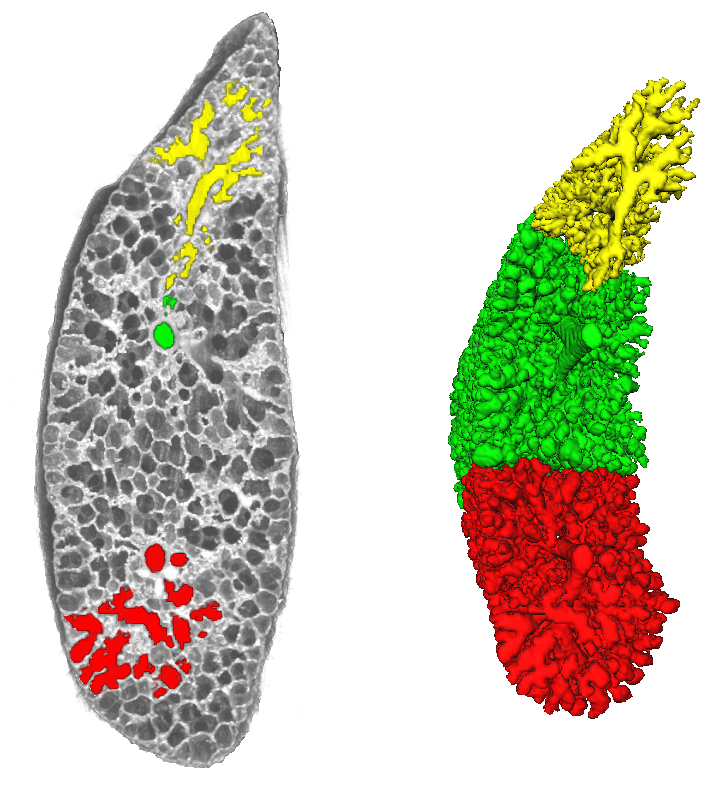
\includegraphics[width=\imagewidth]{img/widefieldscanning/R108C04C-down-merge}};%
			    	\draw[|-|,thick] (547,19) -- (498,775) node [left] {\SI{3.8444}{\milli\meter}};%
				    % 758 px = 3.844 mm > 100 px = 507 um > 99 px = 500um
					\draw[|-|,thick] (\x,\y) -- (198+\x,\y) node [midway,above] {\SI{1}{\milli\meter}};%
				\end{tikzpicture}%
		}%
	\caption{Three dimensional visualization of the distal-medial edge of the right lower lung lobe of a Sprague Dawley rat (same as in figure~\ref{fig:FOV increase overview}). View from the underside of the sample}%
	\label{fig:FOV increase segments}%
\end{figure*}

\subsection{Quality guided protocol selection}
A sequence of 19 protocols with varying quality has been scanned to assess the simulations. The 19 different scans have been chosen according to the MATLAB-plot explained in section~\ref{seq:Image Acquisition}\footnote{generated with ``MATLAB/WideFieldScanning/main.m'' for a protocol with the diameter of \SI{3.8}{mm} and three overlapping subscans}\todo{do we provide the code for reproducible research? or is it ``closed source''?}.

We assessed the image differences for the 19 scanned protocols in such a way that the tiff slices have been binarized using an automated thresholding algorithm method, which chooses the threshold to minimize the intraclass variance of the black and white pixels~\cite{Otsu1979}. The binarization of the images suppresses small variations in the gray values which occur through slight variation in the beam profile during the acquisition of the 57 individual subscans.

The error ($E_{Prot_{i}}$) shown in figure~\ref{fig:NormalizedErrorPlot} has been calculated according to equations~\ref{eq:errorcalculation-a}--\ref{eq:errorcalculation-b}. Using the thresholded slice $i$ of each protocol ($Slice_{Prot_{i}}$) and the corresponding slice $i$ of the gold standard protocol ($Slice_{B_{i}}$) we calculated the absolute difference image ($D_{Prot_{i}}$) of these two slices. The sum of all pixels of this difference image ($D_{Prot_{i}}$) yields the error value ($E_{Prot_{norm_{i}}}$).

\begin{eqnarray}
       D_{Prot_{i}} &=& |Slice_{B_{i}}-Slice_{Prot_{i}}|\label{eq:errorcalculation-a}\\
E_{Prot_{norm_{i}}} &=& \sum_{x}\sum_{y} D_{Prot_{i}}\label{eq:errorcalculation-b}\\
    E_{Prot_{norm}} &=& \overline{E_{Prot_{norm_{i}}}} \pm \sigma(E_{Prot_{norm_{i}}})\label{eq:errorcalculation-c}
\end{eqnarray}

The error value ($E_{Prot_{norm}}$) has been calculated for 205 regularly spaced slices $i=1:5:1024$ of the full dataset (1024 slices). The mean ($\overline{E_{Prot_{norm_{i}}}}$) and standard deviation of the error have been normalized in such a way that the error has been scaled to arbitrary units from 0 to 1.

We see that---as expected---the normalized error grows with decreasing amount of total obtained projections. The simulated scanning quality shown in figure~\ref{fig:2008c-qualityplot} shows the simulated quality to expect from the scan, while figure~\ref{fig:NormalizedErrorPlot} is a plot of the calculated error of the different protocols compared to protocol A, hence the outcome of the experiments using not a simulated phantom, but actual scans of lung tissue. Both the plots for the simulation and the normalized error show the same trend while not being entirely congruent. The simulation shows a exponential decrease in quality, while the calculated, normalized error show a more linear decrease in quality from protocol B towards protocol T.

For protocols with the same total amount of projections, but different configurations of amount of projections for the central and the ring scan (e.g.\ Protocols C and D as well as protocols M and N) we see a difference in the error. This difference arises through the fact that the differing amount of subscans acquired for the central and the subscan add up to the same total amount of projections, but contribute differently to the quality of the reconstruction. The details for those protocols are described in table~\ref{tab:detailsCDMN}. Since the central portions of the sample and the ring portions of the sample cover differently sized areas of the sample, we have expected a different error-value in between the protocols. 

\begin{figure*}
	\centering
		%\documentclass{article}
%\usepackage{tikz,pgfplots}
%\usepackage[pdftex,active,tightpage]{preview}
%\begin{document}
%\begin{preview}
%%%%%%%%%%%%%%%%%%%%%%%%%%%%%%
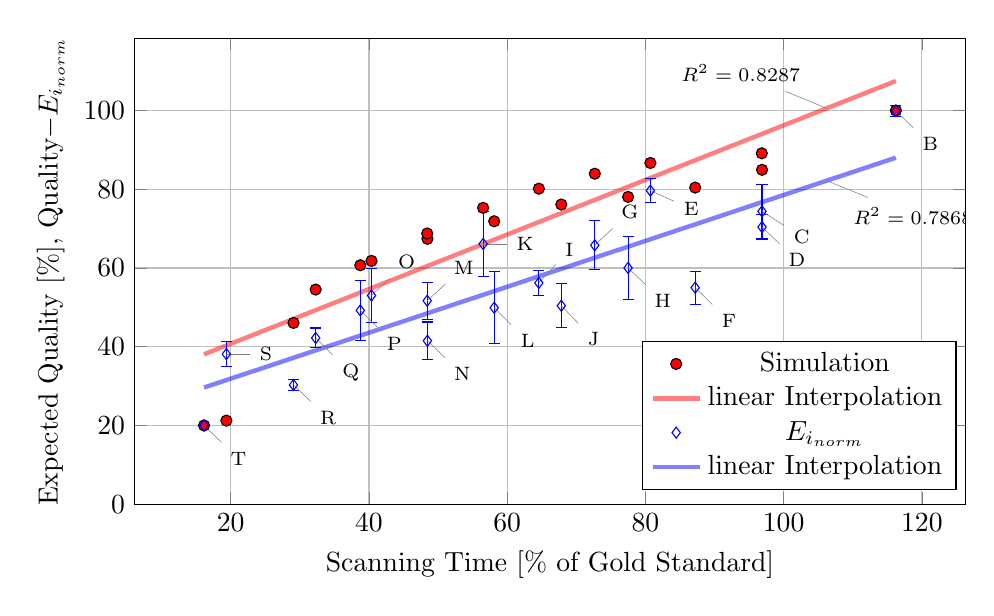
\begin{tikzpicture}

\pgfplotsset{every axis legend/.append style={at={(0.8,0.08)},anchor=base}}

\begin{axis}[%
	xmajorgrids,
  ymajorgrids,
	width=\linewidth,
	height=0.618\linewidth,
	%scale only axis,
	%xmin=0,%xmax=129,
	ymin=0,%ymax=125,
  xlabel={Scanning Time [\%\ of Gold Standard]},%
	ylabel={Expected Quality [\%], Quality$-E_{i_{norm}}$}%
	]

% Protocols
\addplot [ fill=red, only marks, mark = *]
	coordinates{
		(16.14,20)
		(19.37,21.2284)
		(29.08,46.0522)
		(32.29,54.5201)
		(38.75,60.7072)
		(40.37,61.8107)
		(48.46,67.4167)
		(48.43,68.7811)
		(58.12,71.8724)
		(56.52,75.28)
		(67.83,76.1345)
		(64.58,80.1592)
		(77.49,78.0612)
		(72.67,83.9645)
		(87.20,80.4284)
		(80.72,86.6889)
		(96.87,84.9458)
		(96.84,89.1421)
		(116.24,100)
};

\addplot [domain=16.14:116.24,color=red, semitransparent,ultra thick]
	{0.6936*x+26.891}; 

%% Line plot
%\addplot [smooth, solid, semitransparent]
	%coordinates{
		%(16.14,16.8548)
		%(19.37,25.9575)
		%(29.08,46.6567)
		%(32.29,51.7347)
		%(38.75,59.9714)
		%(40.37,61.6854) 
		%(48.46,68.6146)
		%(48.43,68.6305) 
		%(56.52,73.5452)
		%(58.12,74.3455)
		%(64.58,77.1605)
		%(67.83,78.3754)
		%(72.67,80.0091)
		%(77.49,81.5005)
		%(80.72,82.4599)
		%(87.20,84.3973)
		%(96.87,87.719)
%%		(96.87,87.719)
		%(116.24,99.8565)
%};

\addplot [ color=blue, only marks, mark=diamond ]
plot [ error bars/.cd, y dir=both, y explicit ]
    coordinates{
	( 16.14,20.0000) +- (0,0)      % T
	( 19.37,38.1358) +- (0,3.1135) % S
	( 29.08,30.2919) +- (0,1.3958) % R
	( 32.29,42.2255) +- (0,2.5278) % Q
	( 38.75,49.2247) +- (0,7.6789) % P
	( 40.37,53.0181) +- (0,6.8507) % O 
	( 48.46,41.5079) +- (0,4.7824) % N  
	( 48.43,51.6990) +- (0,4.7110) % M
	( 58.12,49.9058) +- (0,9.1839) % L
	( 56.52,66.1100) +- (0,8.1635) % K
	( 67.83,50.4137) +- (0,5.5671) % J
	( 64.58,56.2138) +- (0,3.2329) % I
	( 77.49,60.0243) +- (0,8.0805) % H
	( 72.67,65.7727) +- (0,6.2214) % G
	( 87.20,55.0069) +- (0,4.1882) % F
	( 80.72,79.6708) +- (0,3.0107) % E
	( 96.87,70.4018) +- (0,3.0863) % D
	( 96.87,74.3991) +- (0,6.8125) % C
	(116.24,99.8987) +- (0,1.3487) % B
};

\addplot [domain=16.14:116.24,color=blue, semitransparent,ultra thick]
	{0.5833*x+20.226}; 

\legend{%
	Simulation,%
	linear Interpolation,%
	$E_{i_{norm}}$,%
	linear Interpolation}

% \draw [<-] (axis cs:97.87,74.3991) -- (axis cs:99.87,74.3991) node [anchor=text] {\tiny C}; 
% \draw [<-] (axis cs:97.87,70.4018) -- (axis cs:99.87,70.4018) node [anchor=text] {\tiny D};
% \draw [<-] (axis cs:81.72,79.6708) -- (axis cs:82.72,79.6708) node [anchor=text] {\tiny E};
% \draw [<-] (axis cs:78.49,60.0243) -- (axis cs:79.49,60.0243) node [anchor=text] {\tiny H};
% \draw [<-] (axis cs:65.58,56.2138) -- (axis cs:66.58,56.2138) node [anchor=text] {\tiny I};
% \draw [<-] (axis cs:49.43,51.6990) -- (axis cs:51.43,51.6990) node [anchor=text] {\tiny M};
% \draw [<-] (axis cs:49.46,41.5079) -- (axis cs:51.46,41.5079) node [anchor=text] {\tiny N};

\tikzstyle{every pin}=[pin distance=2ex,font=\scriptsize]
\node[coordinate, pin=below right:{B}] at (axis cs:116.24,99.8987) {}; % B
\node[coordinate, pin=-22.5:{C}] at (axis cs:96.87,74.3991) {}; % C
\node[coordinate, pin=below right:{D}] at (axis cs:96.87,70.4018) {}; % D
\node[coordinate, pin=-5:{E}] at (axis cs:80.72,79.6708) {}; % E
\node[coordinate, pin=below right:{F}] at (axis cs:87.20,55.0069) {}; % F
\node[coordinate, pin=above right:{G}] at (axis cs:72.67,65.7727) {}; % G
\node[coordinate, pin=below right:{H}] at (axis cs:77.49,60.0243) {}; % H
\node[coordinate, pin=above right:{I}] at (axis cs:64.58,56.2138) {}; % I
\node[coordinate, pin=below right:{J}] at (axis cs:67.83,50.4137) {}; % J
\node[coordinate, pin=right:{K}] at (axis cs:56.52,66.1100) {}; % K
\node[coordinate, pin=below right:{L}] at (axis cs:58.12,49.9058) {}; % L
\node[coordinate, pin=above right:{M}] at (axis cs:48.43,51.6990) {}; % M
\node[coordinate, pin=below right:{N}] at (axis cs:48.46,41.5079) {}; % N  
\node[coordinate, pin=above right:{O}] at (axis cs:40.37,53.0181) {}; % O
\node[coordinate, pin=below right:{P}] at (axis cs:38.75,49.2247) {}; % P
\node[coordinate, pin=below right:{Q}] at (axis cs:32.29,42.2255) {}; % Q
\node[coordinate, pin=below right:{R}] at (axis cs:29.08,30.2919) {}; % R
\node[coordinate, pin=right:{S}] at (axis cs:19.37,38.1358) {}; % S
\node[coordinate, pin=below right:{T}] at (axis cs:16.14,20.0000) {}; % T

\node[coordinate, pin=above left:{$R^2=0.8287$}] at (axis cs:106.24,100.5791) {};
\node[coordinate, pin=below right:{$R^2=0.7868$}] at (axis cs:106.24, 82.1958) {};


\end{axis}

\end{tikzpicture}
%%%%%%%%%%%%%%%%%%%%%%%%%%%%%%
%\end{preview}
%\end{document}

%%%%%%%%%%%%%%%%%%%%%%%%%%%%%%
% plot erstellt mit MATLAB-File p:\\MATLAB\WideFieldScan/Paper/wfs_Compare2008c_ErrorPlot.m
% mit FromToTo = 1:5:1024
% sowie matlab2tikz
% Daten
%%%%%%%%%%Time =
%%%%%%%%%%  Columns 1 through 12
%%%%%%%%%%
%%%%%%%%%%   13.75   16.50   24.77   27.50   33   34.38   41.27   41.25   49.50   48.14   57.77   55
%%%%%%%%%%
%%%%%%%%%%  Columns 13 through 19
%%%%%%%%%%
%%%%%%%%%%   66   61.89   74.27   68.75   82.50   82.50   99.01
%MeanCumulativeError =
%
%  Columns 1 through 12
%
%   20.0000   38.1358   30.2919   42.2255   49.2247   53.0181   41.5079   51.6990   49.9058   66.1100   50.4137   56.2138
%
%  Columns 13 through 19
%
%   60.0243   65.7727   55.0069   79.6708   70.4018   74.3991   99.8987
%
%
%StandardDeviationofCumulativeError =
%
%  Columns 1 through 12
%
%         0    3.1135    1.3958    2.5278    7.6789    6.8507    4.7824    4.7110    9.1839    8.1635    5.5671    3.2329
%
%  Columns 13 through 19
%
%    8.0805    6.2214    4.1882    3.0107    3.0863    6.8125    1.3487
%%%%%%%%%%%%%%%%%%%%%%%%%%%%%%
	\caption{Plot of normalized Error ($E_{norm}$ for the 19 scanned protocols. The normalized Error has been calculated in such a way that we calculated the difference image for Protocol 'x' compared to Protocol 'A',  and . The error bars for each protocol show the standard deviation of the error which was calculated for 205 of the 1024 slices for each protocol. Note that the error is plotted inversely, so the axes of this plot and the plot in figure~\ref{fig:2008c-qualityplot} are directly comparable.}
	\label{fig:NormalizedErrorPlot}
\end{figure*}

\begin{table*}%
	\centering
	\caption{Details of amount of projections for protocols C vs.\ D and M vs.\ N}
	\begin{tabular}{rcccc}
		\toprule
							& C 	& D 	& M 	& N \\
		\midrule
		Central scan		& 2622 	& 4370	& 1311 	& 2185 \\
		Ring scan	 		& 5244 	& 4370  & 2622 	& 2185 \\
		\midrule
		total Projections	& 13110	& 13110	& 6555	& 6555 \\
		\bottomrule
	\end{tabular}  
	\label{tab:detailsCDMN}
\end{table*}

Figure~\ref{fig:NormalizedErrorPlot} confirms this finding. For a comparable total amount of recorded projections, the quality of the dataset with reduced projections is lower than when an equal amount of projections has been recorded for all three subscans\todo{compare O/P, M/N, I/J, E/H, C/D in depth!}.

\subsubsection{Comparison of protocols obtained with quality-guided protocol selection}
The 19 different protocols which have been obtained from the same sample have been three dimensionally visualized and analyzed using MeVisLab (Version 1.6.1 (2008-09-21 Release), MeVis Medical Solutions AG, Bremen, Germany). Using a region growing algorithm~\cite{wiki:regiongrowing}, airway segments have been extracted from the tomographic dataset. To be able to compare the extracted airway segments (segments for two protocols are shown in figures~\ref{subfig:BvsToverviewB}--\ref{subfig:BvsTsegmentT}) we used exactly the same seed points for all protocols. Since the histograms of the slices from the different protocols were not completely equal, slightly different threshold values have been used to define if a voxel is include in the airway segment or not. All these threshold have been chosen in such a way that they were placed at the same location in the histogram\todo{do we need to show this, or is explanation enough?}.

\begin{figure*}
	\centering
	\pgfmathsetlength{\imagewidth}{\imsize}          % desired displayed width of image
	\pgfmathsetlength{\imagescale}{\imagewidth/1594} % pixel width of imagefile used
	\subfloat[Overview Protocol B]{%
		\label{subfig:BvsToverviewB}%
	    \begin{tikzpicture}[x=\imagescale,y=-\imagescale]
	    \def\x{225}
    	\def\y{825}
      		\node[anchor=north west,inner sep=0pt,outer sep=0pt] at (0,0)
			{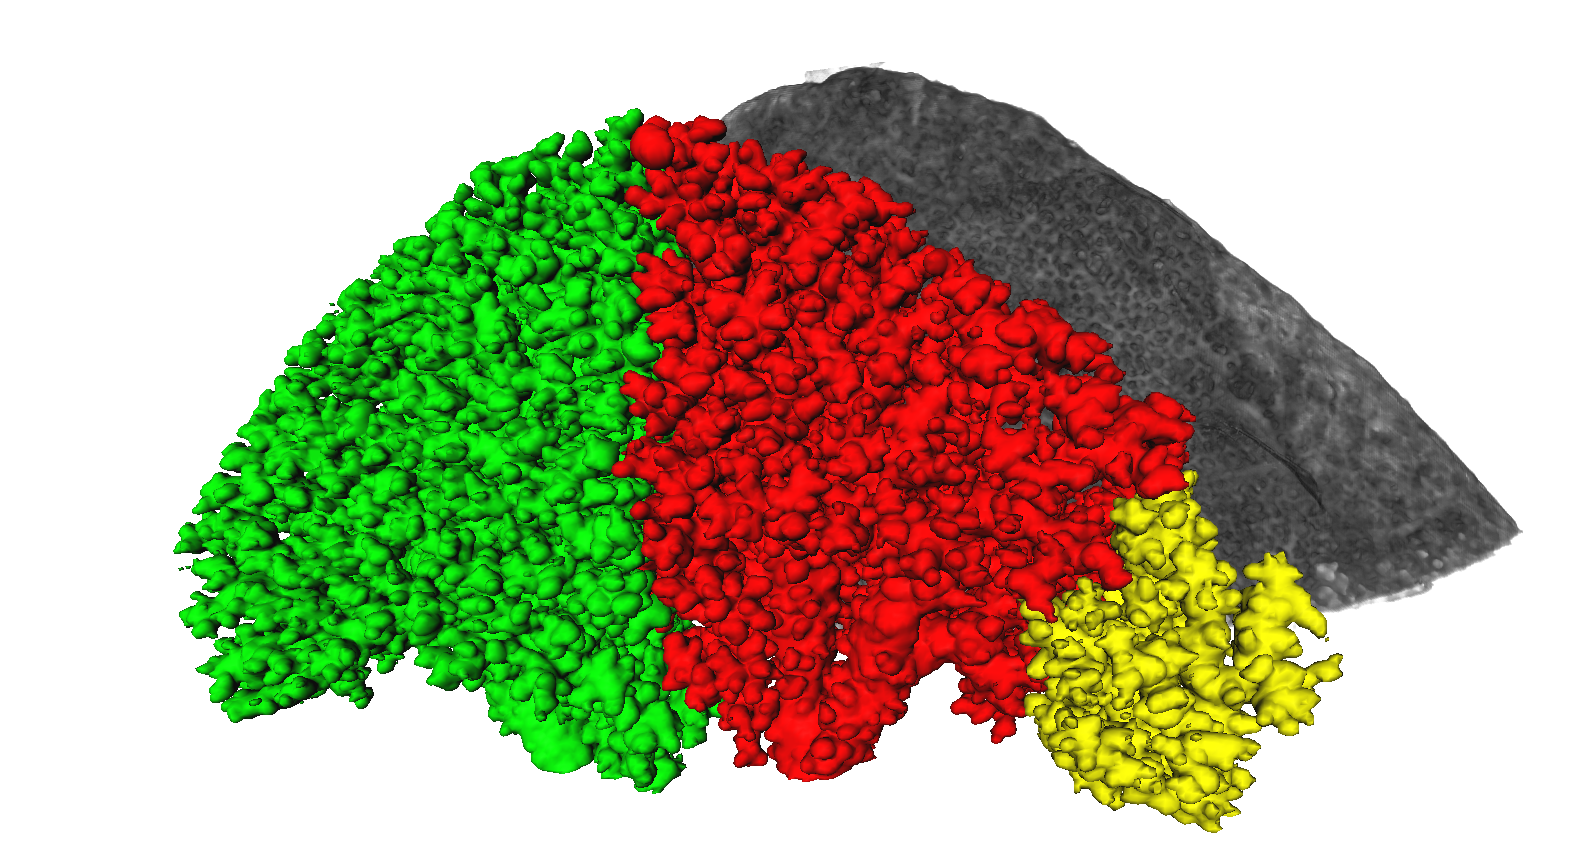
\includegraphics[width=\imagewidth]{img/comparisonBvsT/R108C21_overview_B}};
			% 1204 px = 3.844 mm > 100 px = 319 um > 157 px = 500 um
		    \draw[|-|,thick] (174,550) -- (1352,797) node [midway,above] {\SI{3.8444}{\milli\meter}}; 
			\draw[|-|,thick] (\x,\y) -- (\x+157,\y) node [right] {\SI{500}{\micro\meter}};
    	\end{tikzpicture}%
		}%
	\subfloat[Overview Protocol T]{%
		\label{subfig:BvsToverviewT}%
		\begin{tikzpicture}[x=\imagescale,y=-\imagescale]
		\def\x{225}
    	\def\y{825}
    		\node[anchor=north west,inner sep=0pt,outer sep=0pt] at (0,0)
			{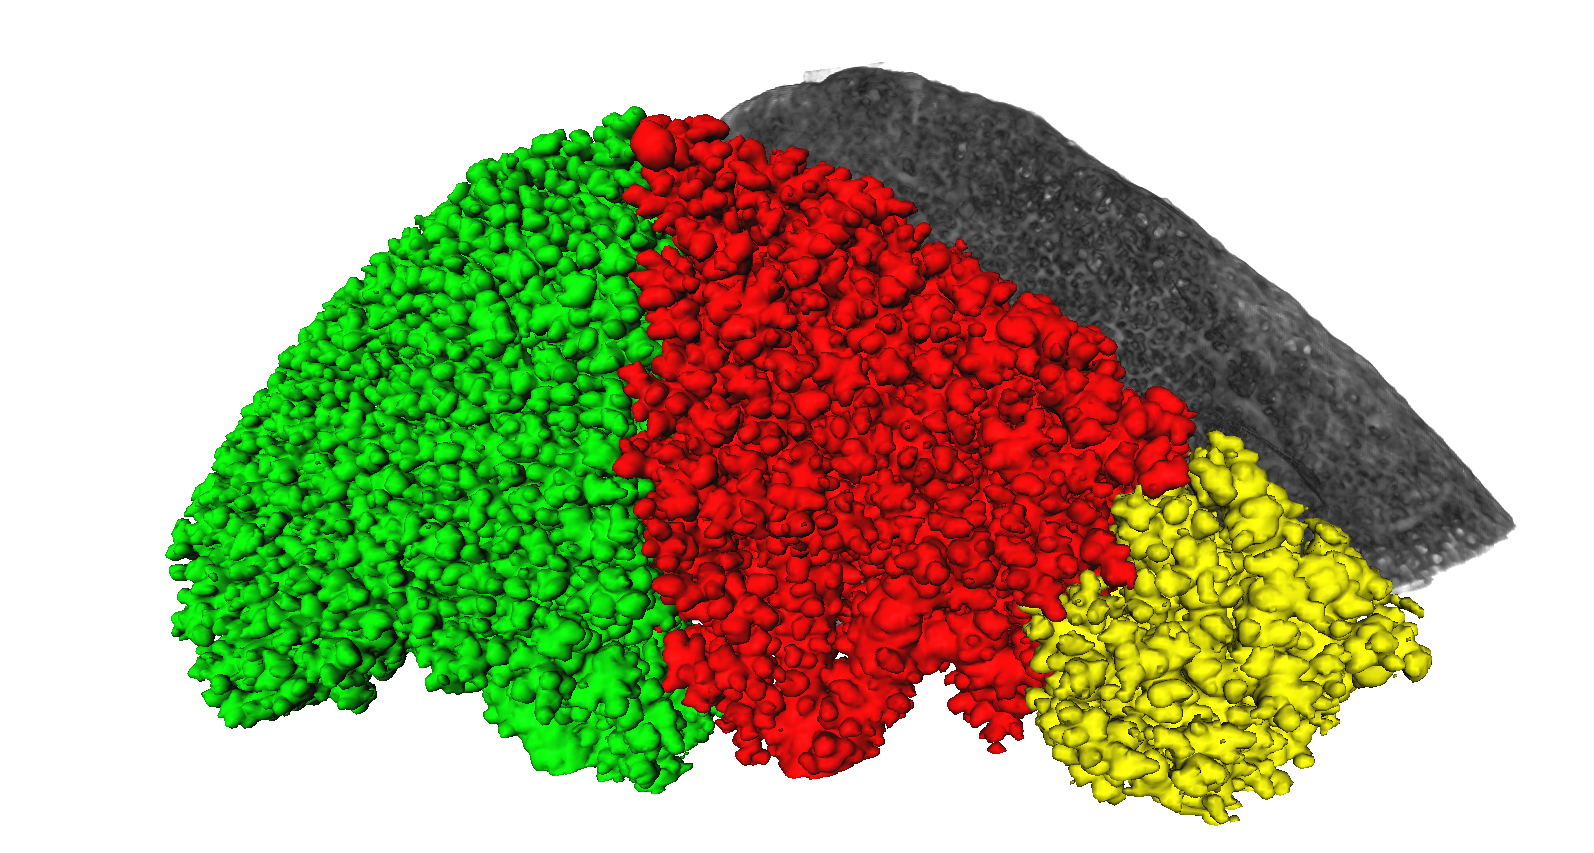
\includegraphics[width=\imagewidth]{img/comparisonBvsT/R108C21_overview_T}};
			% 1204 px = 3.844 mm > 100 px = 319 um > 157 px = 500 um
		    \draw[|-|,thick] (174,550) -- (1352,797) node [midway,above] {\SI{3.8444}{\milli\meter}};
			\draw[|-|,thick] (\x,\y) -- (\x+157,\y) node [right] {\SI{500}{\micro\meter}};
    	\end{tikzpicture}%
		}\\
	\subfloat[Segmented airways for protocol B]{%
		\label{subfig:BvsTsegmentB}%
		\begin{tikzpicture}[x=\imagescale,y=-\imagescale]
		\def\x{225}
    	\def\y{675}
      		\node[anchor=north west,inner sep=0pt,outer sep=0pt] at (0,0)
			{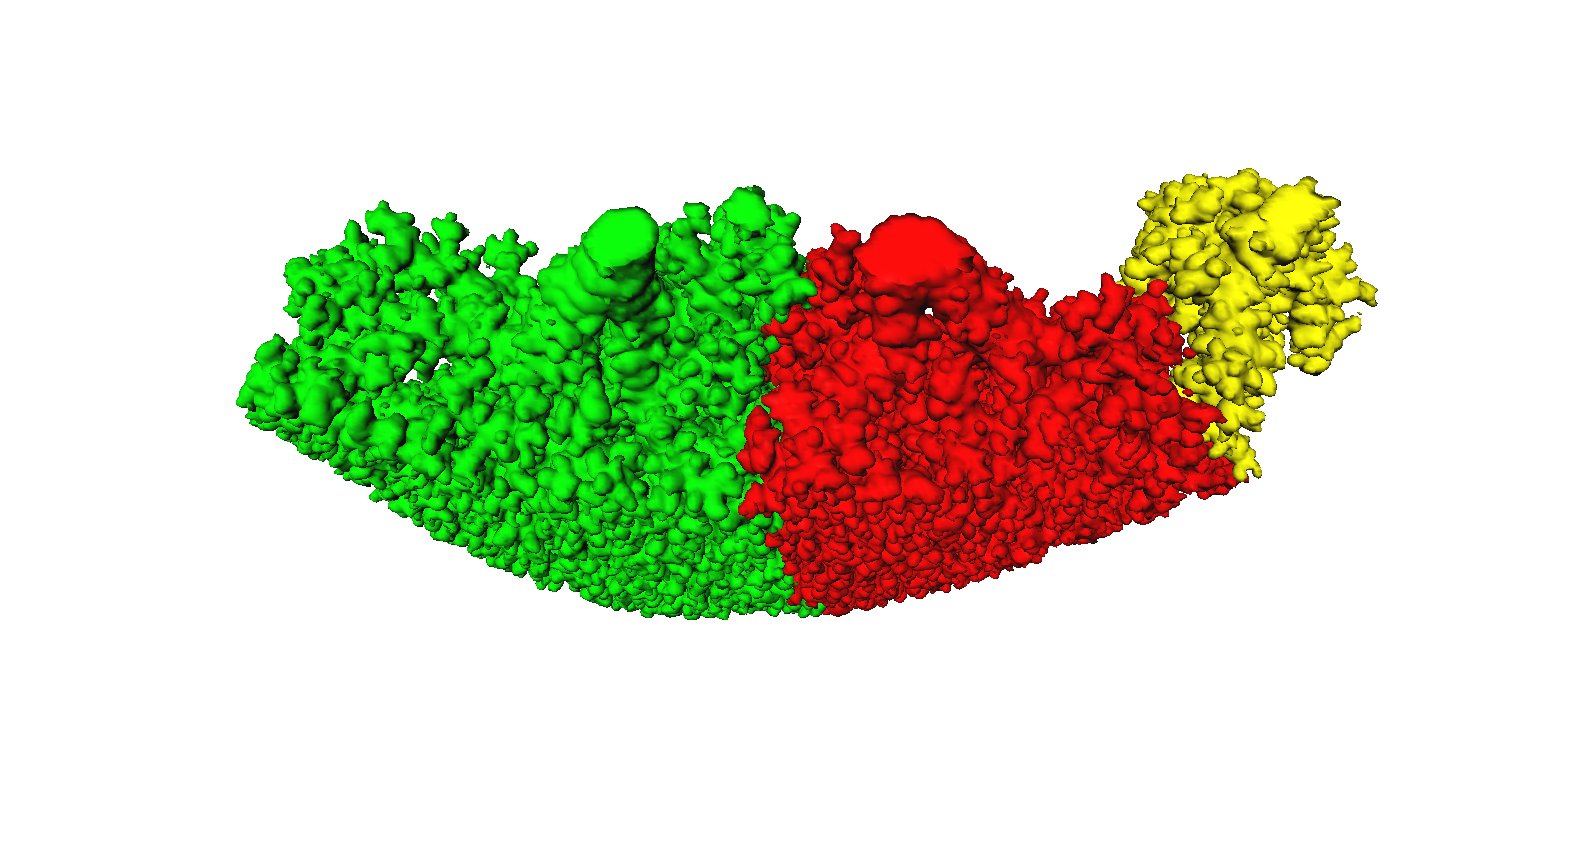
\includegraphics[width=\imagewidth]{img/comparisonBvsT/R108C21_underside_iso_B}};
			% 1341 px = 3.844 mm > 100 px = 287 um > 174 px = 500 um
		    \draw[|-|,thick] (183,288) -- (1523,279) node [midway,above] {\SI{3.8444}{\milli\meter}};
			\draw[|-|,thick] (\x,\y) -- (\x+174,\y) node [right] {\SI{500}{\micro\meter}};
    	\end{tikzpicture}%
		}%
	\subfloat[Segmented airways for protocol T]{%
		\label{subfig:BvsTsegmentT}%
		\begin{tikzpicture}[x=\imagescale,y=-\imagescale]
		\def\x{225}
    	\def\y{675}
			\node[anchor=north west,inner sep=0pt,outer sep=0pt] at (0,0)
			{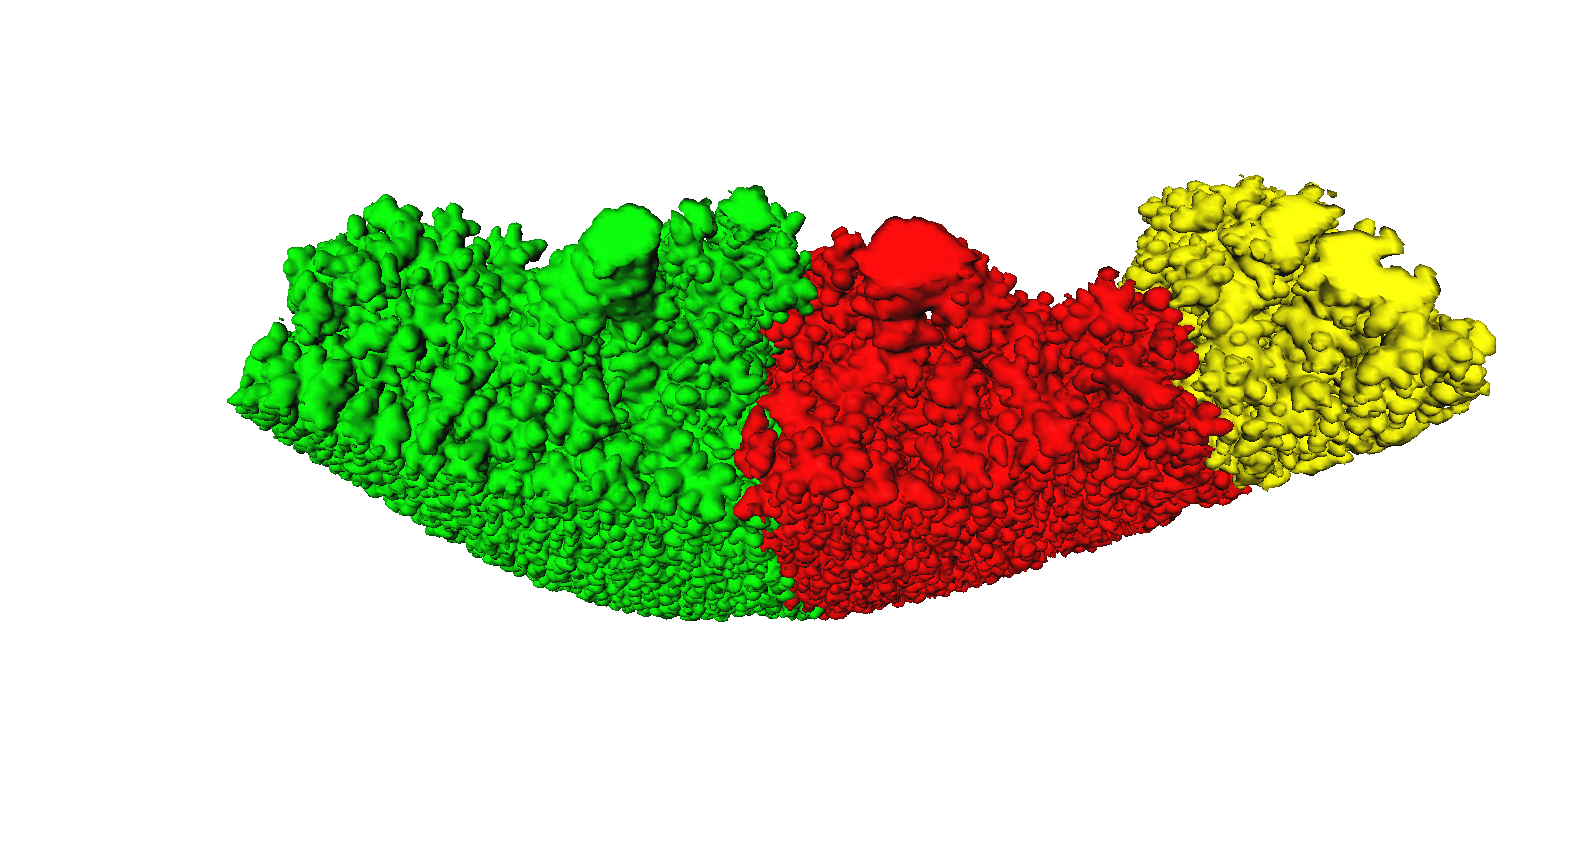
\includegraphics[width=\imagewidth]{img/comparisonBvsT/R108C21_underside_iso_T}};
			% 1341 px = 3.844 mm > 100 px = 287 um > 174 px = 500 um
		    \draw[|-|,thick] (183,288) -- (1523,279) node [midway,above] {\SI{3.8444}{\milli\meter}};
			\draw[|-|,thick] (\x,\y) -- (\x+174,\y) node [right] {\SI{500}{\micro\meter}};
		\end{tikzpicture}%
		}\\
	\pgfmathsetlength{\imagescale}{\imagewidth/2712} % pixel width of imagefile used		
	\subfloat[Slice 1024 of dataset for protocol B, reconstructed from 5244 merged projections.]{%
		\label{subfig:BvsTsliceB}%
		\begin{tikzpicture}[x=\imagescale,y=-\imagescale]
		\def\x{150}
    	\def\y{150}    		
      		\node[anchor=north west,inner sep=0pt,outer sep=0pt] at (0,0)
			{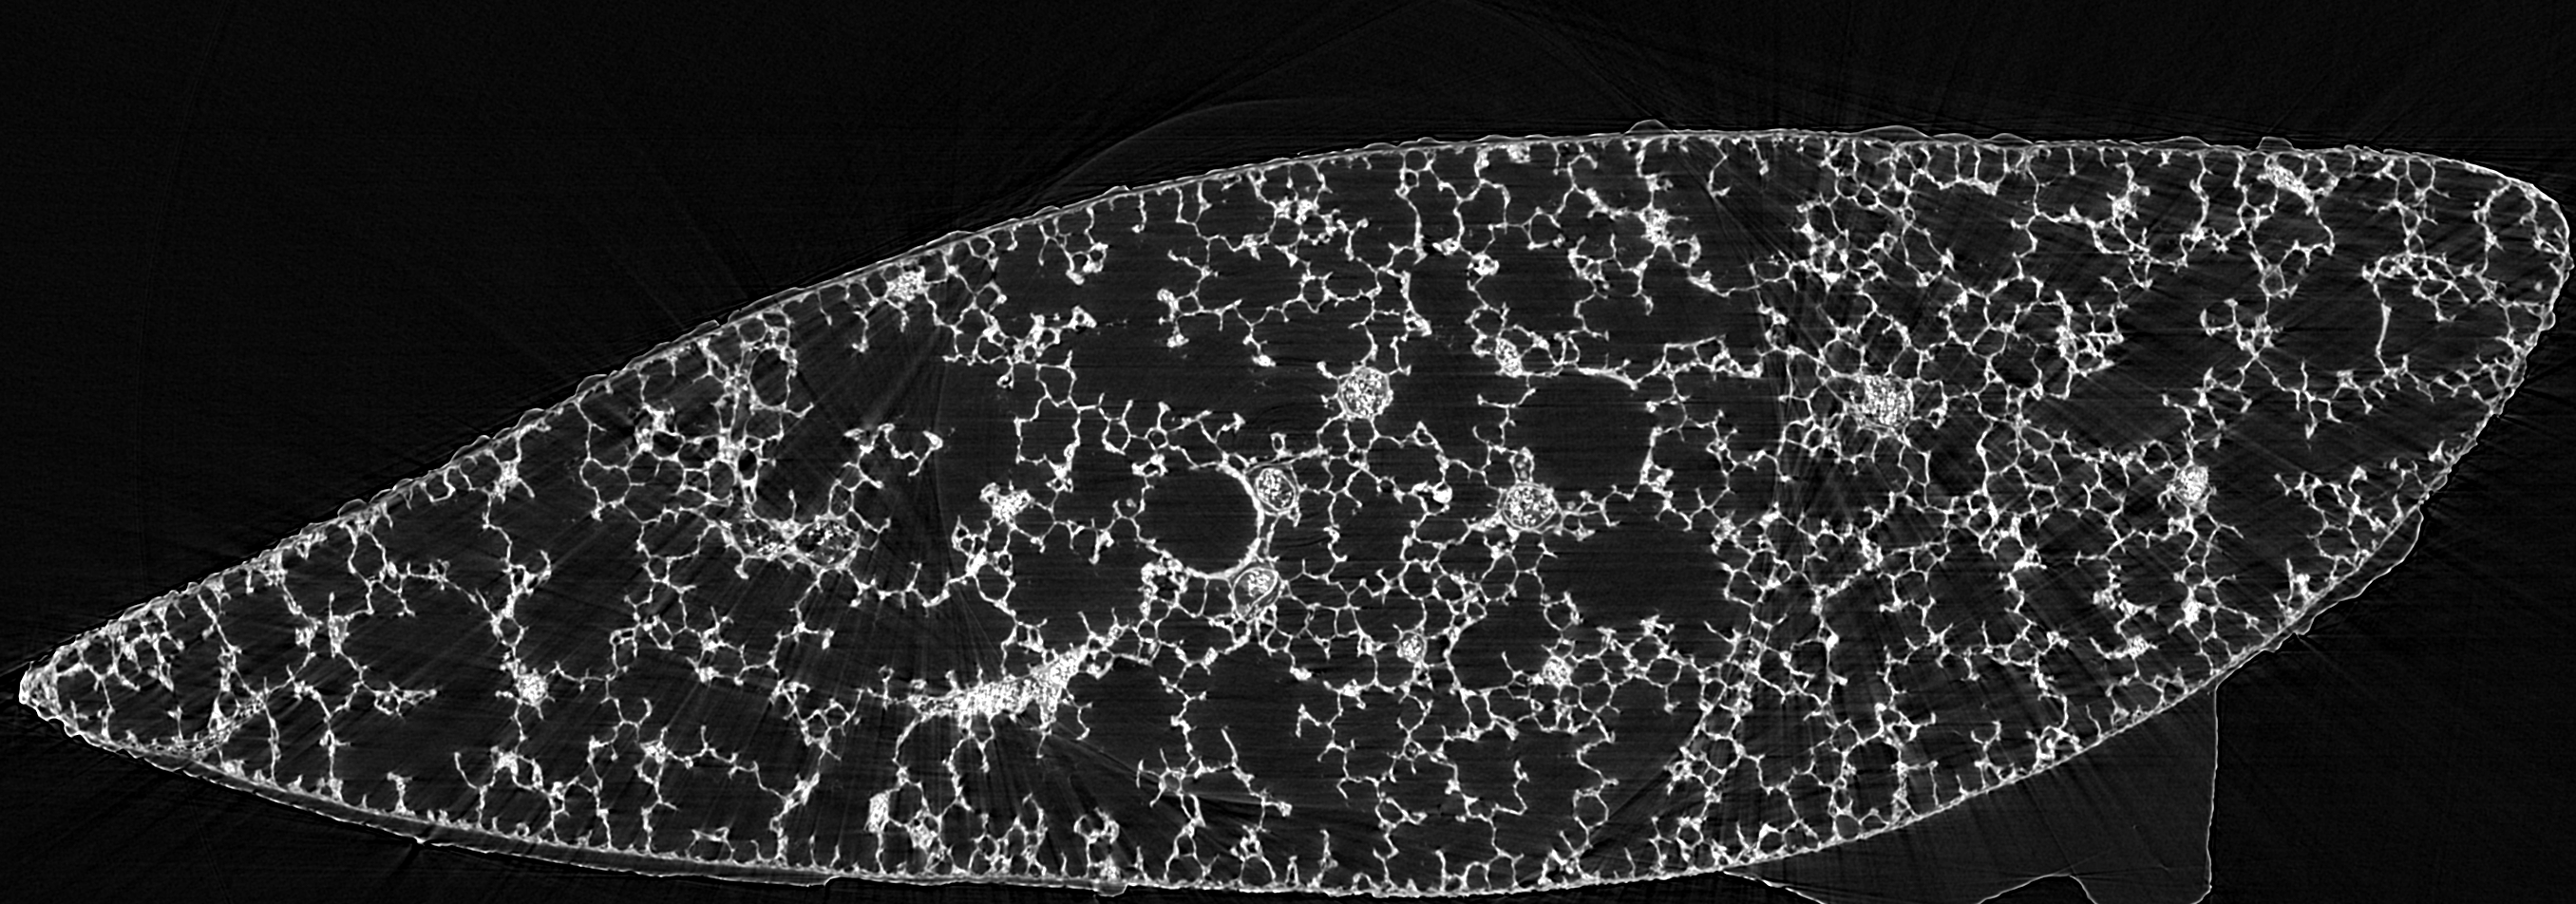
\includegraphics[width=\imagewidth]{img/protocols/R108C21Cb_mrg1024}};
			% 2710 px = 3.844 cm > 100 px = 142 um > 352 px = 500 um
		    \draw[|-|,color=white,thick] (10,500) -- (2702,500) node [midway,above] {\SI{3.8444}{\milli\meter}};
			\draw[|-|,color=white,thick] (\x,\y) -- (352+\x,\y) node [right] {\SI{500}{\micro\meter}};
    	\end{tikzpicture}%
		}%
	\subfloat[Slice 1024 of dataset for protocol T, reconstructed from 874 merged projections.]{%
		\label{subfig:BvsTsliceT}%
		\begin{tikzpicture}[x=\imagescale,y=-\imagescale]
		\def\x{150}
    	\def\y{150}  
      		\node[anchor=north west,inner sep=0pt,outer sep=0pt] at (0,0)
			{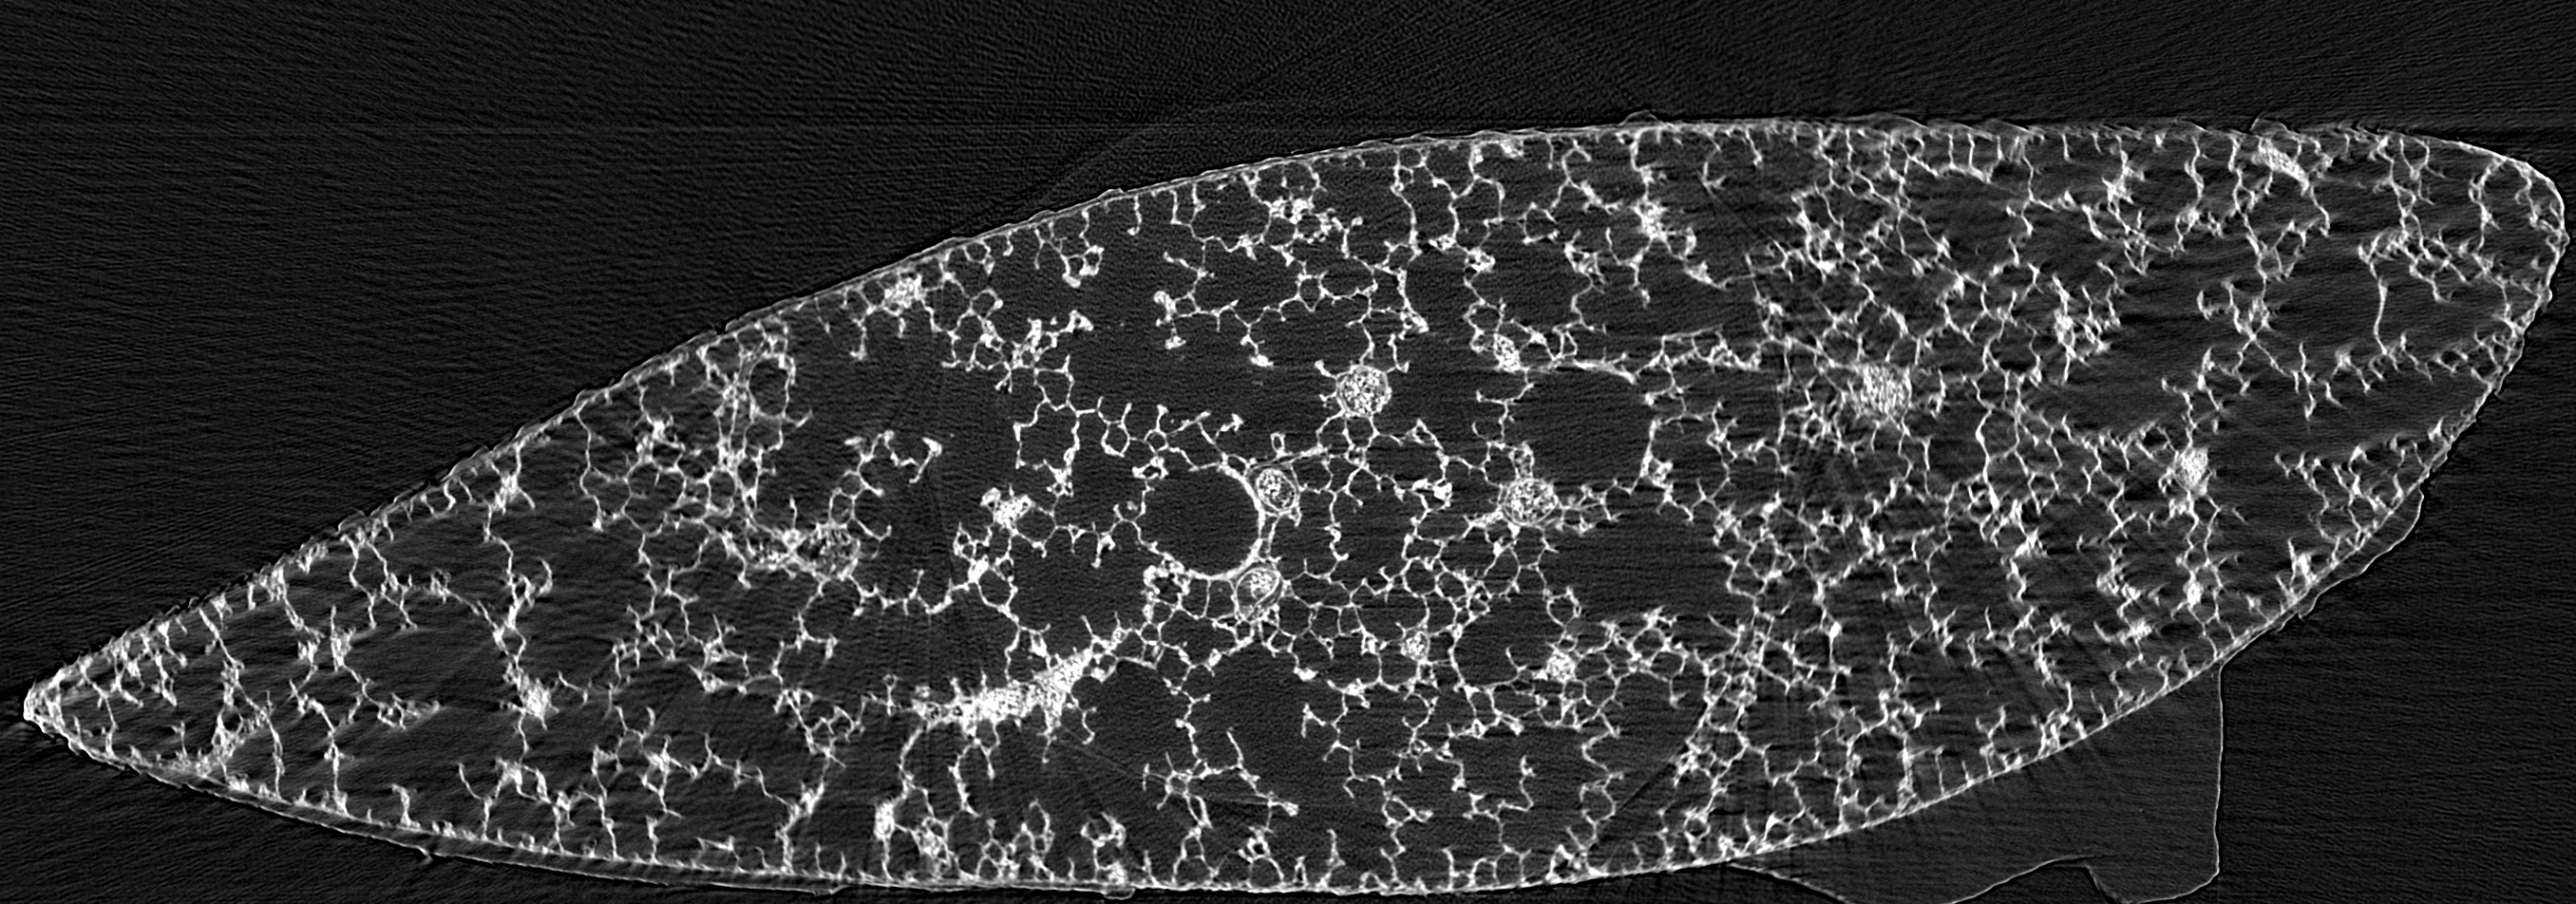
\includegraphics[width=\imagewidth]{img/protocols/R108C21Ct_mrg1024}};
			% 2710 px = 3.844 cm > 100 px = 142 um > 352 px = 500 um
		    \draw[|-|,color=white,thick] (10,500) -- (2702,500) node [midway,above] {\SI{3.8444}{\milli\meter}};
		    \draw[|-|,color=white,thick] (\x,\y) -- (352+\x,\y) node [right] {\SI{500}{\micro\meter}};
    	\end{tikzpicture}%
		}\\
	\caption{Comparison of protocols B and T. Top row: overview. Center row: view of the isosurfaces of the segmented airways. Bottom row: Slices}%
	\label{fig:BvsT}%
\end{figure*}

The two protocols shown in figure~\ref{fig:BvsT} are the two extremes of the 19 obtained protocols. The dataset shown on the left (B) has been reconstructed from 5244 merged projection images, the dataset shown on the right (T) has been reconstructed using only 874 merged slices. Albeit we have scanned protocol T while violating the sampling theorem, both samples still look nearly identical in the three dimensional visualization. Except for small differences at the most lateral parts of the sample (yellow segment) the segmented airways are identical, even if the scanning time of protocol T has been reduced to \SI{14}{\percent} of the scanning time of protocol B\todo{elaborate a bit more on this\ldots}.

\subsubsection{Iteration to even bigger fields of view}
As a proof of concept we have extended the FOV from three to five subscans. We have been able to reconstruct a sample with size of approximately 0.4$\times$3.4$\times$\SI{0.7}{\milli\meter} at a voxel side length of \SI{0.7}{\micro\meter}. A visualization of such a lung tissue slab is shown in figure~\ref{fig:LungSlabSophie}\todo{Compare the red and green cube $\rightarrow$ artefacts at lateral parts}.

\begin{figure*}
	\renewcommand{\imsize}{\textwidth}
	\pgfmathsetlength{\imagewidth}{\imsize} 		 % desired displayed width of image
	\pgfmathsetlength{\imagescale}{\imagewidth/1589} % 1589*728 = width of imagefile used below
	\newcommand{\startx}{982} %= 1589*.618
	\newcommand{\starty}{655} %= 728*.9
	\centering
	\subfloat[]{
		\begin{tikzpicture}[x=\imagescale,y=-\imagescale]
 			\node[anchor=north west,inner sep=0pt,outer sep=0pt] at (0,0)
 			{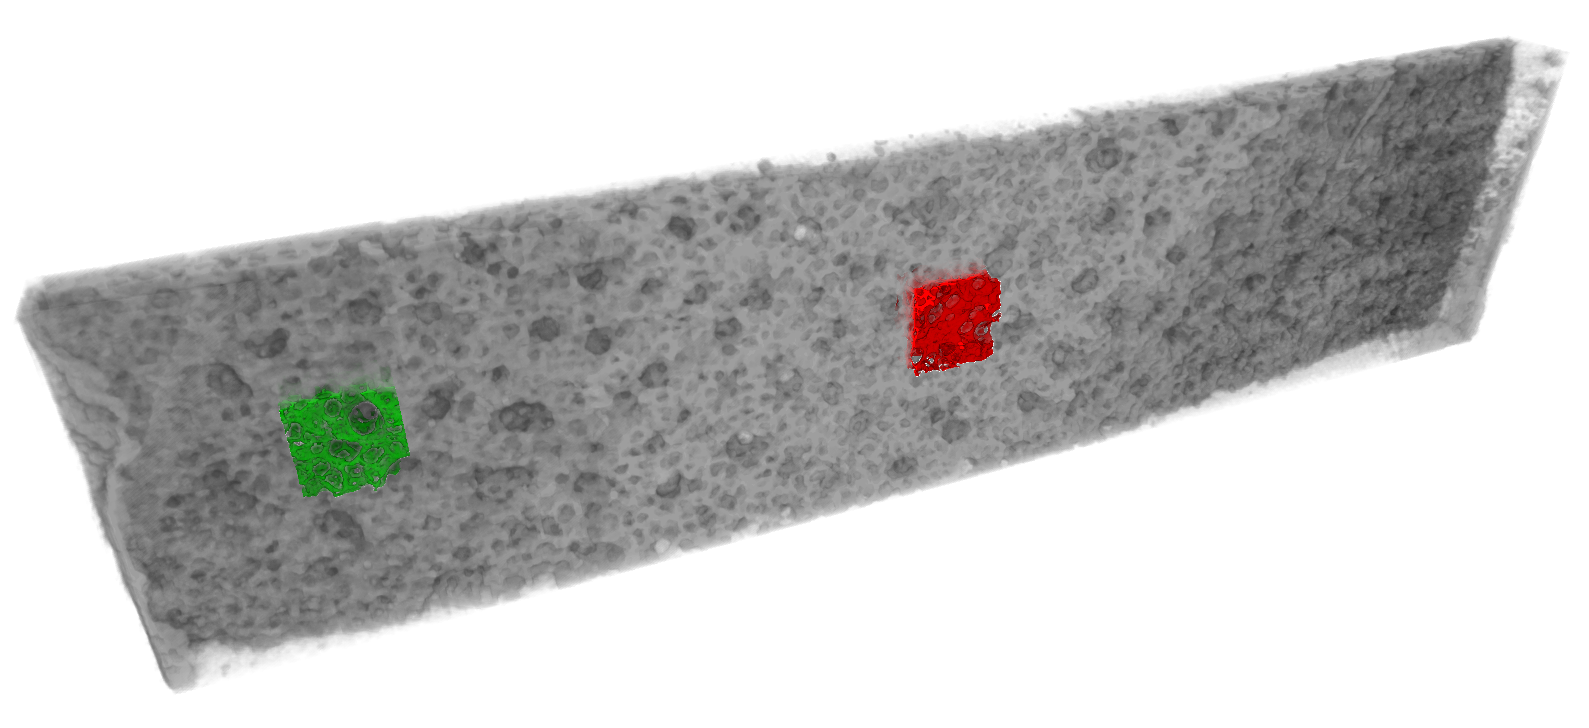
\includegraphics[width=\imagewidth]{img/sophie/full}};
 			\draw[|-|](\startx-808,\starty) -- (\startx+500,\starty) node[midway,above] {\SI{3.3978}{\milli\meter}}; % 4854px * 0.7 um/px = 3.3978 mm
	 	\end{tikzpicture}
	 	\label{subfig:LungSlab}
		}
	\renewcommand{\imsize}{.25\linewidth}
	\pgfmathsetlength{\imagewidth}{\imsize} % desired displayed width of image
	\pgfmathsetlength{\imagescale}{\imagewidth/902} % 1543*928 = width of imagefile used below
	\renewcommand{\startx}{557} %= 902*.618
	\renewcommand{\starty}{802} %= 891*.9
	\subfloat[]{%
		\begin{tikzpicture}[x=\imagescale,y=-\imagescale]
			\node[anchor=north west,inner sep=0pt,outer sep=0pt] at (0,0)
 			{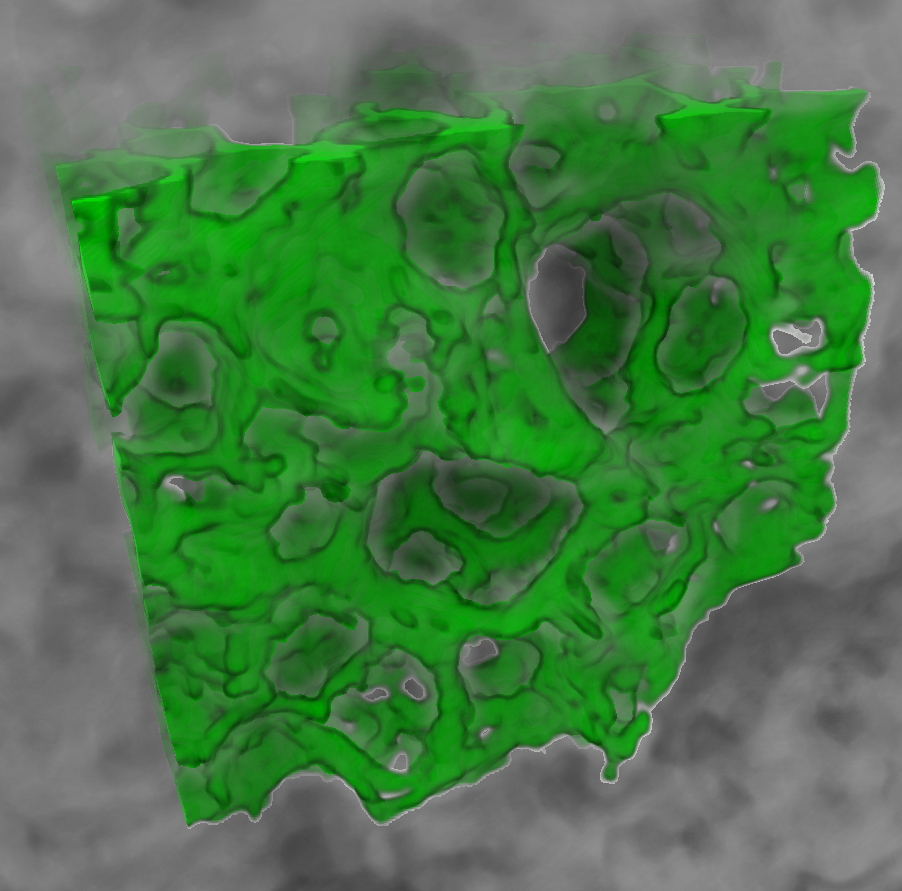
\includegraphics[width=\imagewidth]{img/sophie/crop-green-background}};
 			\draw[|-|] (\startx+0,\starty) -- (\startx+200,\starty) node[midway,above] {\SI{179.2}{\micro\meter}}; % cube with 256 px = 179.2 um
	 	\end{tikzpicture}%
	 	\label{subfig:LungSlabDetailsGreenBG}%
		}
	\subfloat[]{%
		\begin{tikzpicture}[x=\imagescale,y=-\imagescale]
			\node[anchor=north west,inner sep=0pt,outer sep=0pt] at (0,0)
 			{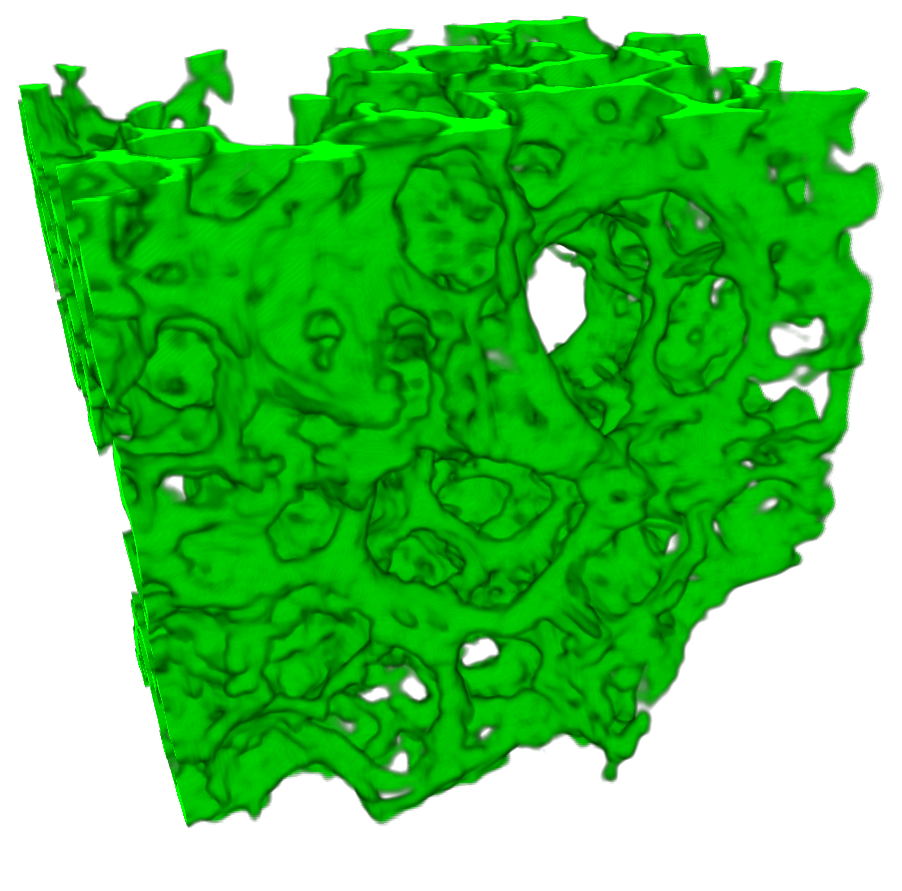
\includegraphics[width=\imagewidth]{img/sophie/crop-green}};
 			\draw[|-|] (\startx+0,\starty) -- (\startx+200,\starty) node[midway,above] {\SI{179.2}{\micro\meter}}; % cube with 256 px = 179.2 um
	 	\end{tikzpicture}%
	 	\label{subfig:LungSlabDetailsGreen}%
		}%
	\subfloat[]{%
		\begin{tikzpicture}[x=\imagescale,y=-\imagescale]
			\node[anchor=north west,inner sep=0pt,outer sep=0pt] at (0,0)
 			{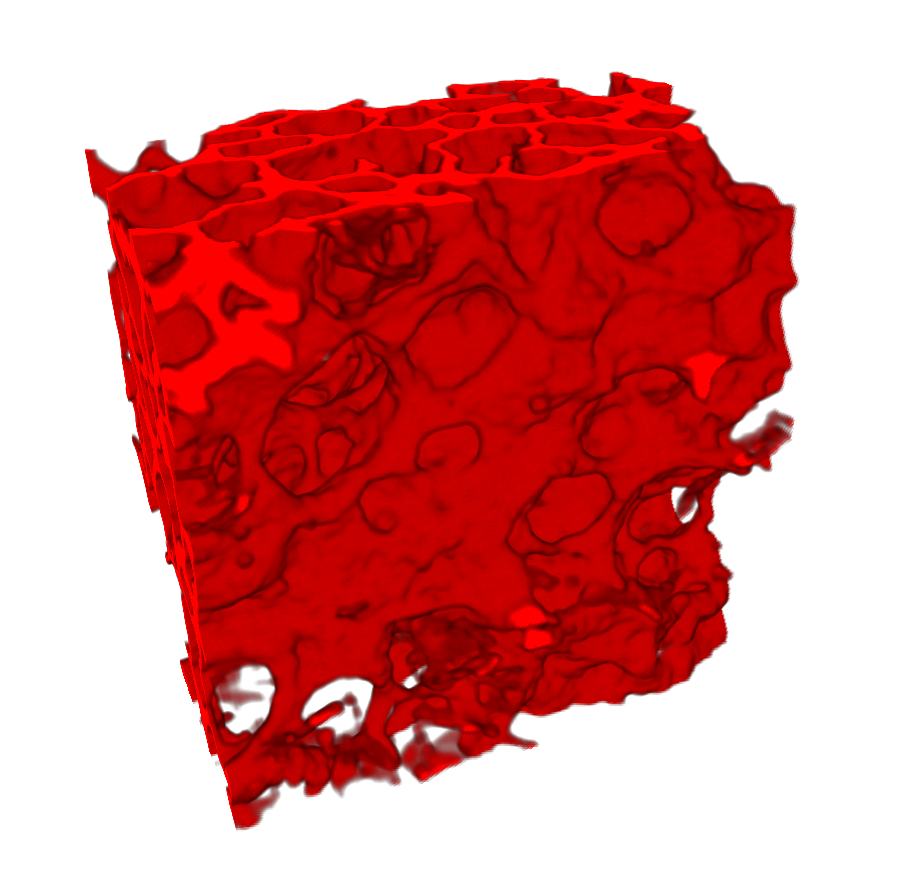
\includegraphics[width=\imagewidth]{img/sophie/crop-red}};
 			\draw[|-|] (\startx+0,\starty) -- (\startx+200,\starty) node[midway,above] {\SI{179.2}{\micro\meter}}; % cube with 256 px = 179.2 um
	 	\end{tikzpicture}%
	 	\label{subfig:LungSlabDetailsRed}%
		}
	\subfloat[]{%
		\begin{tikzpicture}[x=\imagescale,y=-\imagescale]
			\node[anchor=north west,inner sep=0pt,outer sep=0pt] at (0,0)
 			{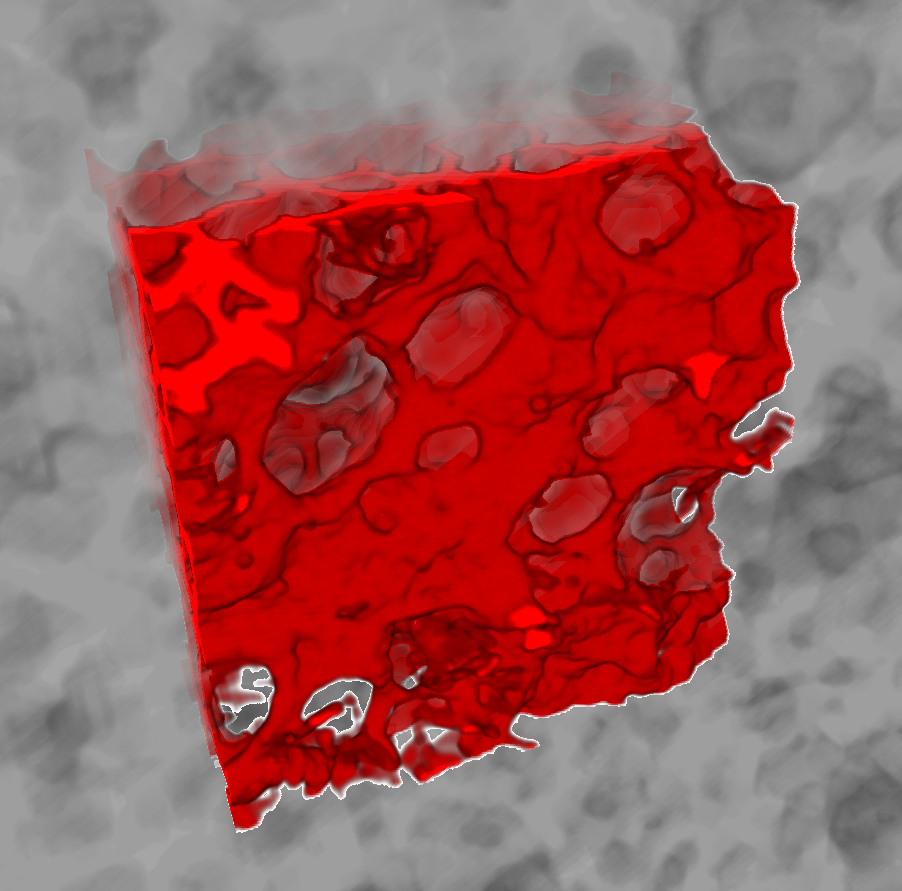
\includegraphics[width=\imagewidth]{img/sophie/crop-red-background}};
 			\draw[|-|] (\startx+0,\starty) -- (\startx+200,\starty) node[midway,above] {\SI{179.2}{\micro\meter}}; % cube with 256 px = 179.2 um
	 	\end{tikzpicture}%
	 	\label{subfig:LungSlabDetailsRedBG}%
		}
	\caption{Visualization of lung tissue slab: %
		\subref{subfig:LungSlab}: Three dimensional volume rendering of slab of lung tissue with a size of 554$\times$4854$\times$1024 pixels at a voxel side length of \SI{0.7}{\micro\meter}. Both inset cubes have a side length of 256 pixels and were automatically segmented using a region growing algorithm. 
 		\subref{subfig:LungSlabDetailsGreenBG}: Close-up of inset cube at an outer position in the sample, including the background tissue. % 
 		\subref{subfig:LungSlabDetailsGreen}: Close-up of inset cube at an outer position in the sample. Albeit we have been able to automatically segment the lung tissue, segmentation artifacts are visible. Single alveoli can be distinguished. %
 		\subref{subfig:LungSlabDetailsRed}: Close-up of inset cube at a central position in the sample. Single alveoli are clearly visible. %
 		\subref{subfig:LungSlabDetailsRedBG}: Close-up of inset cube at a central position in the sample, including the background tissue. %
	}
	\label{fig:LungSlabSophie}%
\end{figure*}